%  !TeX  root  =  user_guide.tex  

%\section{GRASS GIS Integration}\label{sec:grass}\index{GRASS}
\chapter{Intégration du SIG \grass}\label{sec:grass}\index{\grass}

% when the revision of a section has been finalized, 
% comment out the following line:
%\updatedisclaimer

%The \grass plugin provides access to \grass GIS~\cite{\grassweb} databases and 
%functionalities. This includes visualization of \grass raster and vector 
%layers, digitizing vector layers, editing vector attributes, creating new 
%vector layers and analysing \grass 2D and 3D data with more than 300 \grass 
%modules.

L'extension \grass fournit un accès aux bases de données et aux fonctionnalités de \grass.  Cela inclut la visualisation des couches d'informations \grass raster et vecteur,  la numérisation de couches vecteurs, l'édition des attributs des couches d'informations vecteurs,  la création de nouvelles couches et l'analyse 2D et 3D grâce à l'accès à près de 300 modules \grass. 

%In this Section we'll introduce the plugin functionalities and give some 
%examples on managing and working with \grass data. Following main features 
%are provided with the toolbar menu, when you start the \grass plugin, as 
%described in Section~\ref{sec:starting_grass}:

Dans cette section, nous présenterons les fonctionnalités de l'extension et nous donnerons des exemples sur la manière de gérer et de travailler avec des données \grass. Les fonctionnalités principales suivantes sont fournies dans la barre de menu lorsque vous lancez l'extension \grass, comme décrit dans la section ~\ref{sec:starting_grass}:
 
\begin{itemize}[label=--]
%\item \toolbtntwo{grass_open_mapset}{Open mapset}
%\item \toolbtntwo{grass_new_mapset}{New mapset}
%\item \toolbtntwo{grass_close_mapset}{Close mapset}
%\item \toolbtntwo{grass_add_vector}{Add \grass vector layer}
%\item \toolbtntwo{grass_add_raster}{Add \grass raster layer}
%\item \toolbtntwo{grass_new_vector_layer}{Create new \grass vector}
%\item \toolbtntwo{grass_edit}{Edit \grass vector layer}
%\item \toolbtntwo{grass_tools}{Open \grass tools}
%\item \toolbtntwo{grass_shell}{Open \grass Shell}
%\item \toolbtntwo{grass_region}{Display current \grass region} 
%\item \toolbtntwo{grass_region_edit}{Edit current \grass region}
\item \toolbtntwo{grass_open_mapset}{Ouvrir le jeu de données}
\item \toolbtntwo{grass_new_mapset}{Nouveau jeu de données}
\item \toolbtntwo{grass_close_mapset}{Fermer le jeu de données}
\item \toolbtntwo{grass_add_vector}{Ajouter une couche vectorielle \grass}
\item \toolbtntwo{grass_add_raster}{Ajouter une couche raster \grass}
\item \toolbtntwo{grass_new_vector_layer}{Créer une nouvelle couche vectorielle \grass}
\item \toolbtntwo{grass_edit}{Éditer une couche vectorielle \grass}
\item \toolbtntwo{grass_tools}{Ouvrir les outils \grass}
%\item \toolbtntwo{grass_shell}{Ouvrir le shell \grass}
\item \toolbtntwo{grass_region}{Afficher la région courante \grass} 
\item \toolbtntwo{grass_region_edit}{Éditer la région courante \grass}
\end{itemize}

%\section{Starting the \grass plugin}\label{sec:starting_grass}
\section{Lancer l'extension \grass}\label{sec:starting_grass}
%\index{\grass!starting \qg}
\index{\grass!Démarrage de \qg}

%To use \grass functionalities and/or visualize \grass vector and raster layers 
%in \qg, you must select and load the \grass plugin with the Plugin Manager. 
%Therefore click the menu \mainmenuopt{Plugins} > \mainmenuopt{Manage Plugins}, 
%select \dropmenuopt{\grass} and click \button{OK}.

Pour pouvoir utiliser les fonctionnalités de \grass et/ou visualiser des données vecteurs ou raster dans \qg, 
vous devez sélectionner et charger l'extension \grass à l'aide du gestionnaire d'extensions. 
Pour le faire cliquez sur le menu \mainmenuopt{Extensions} > \mainmenuopt{Gestionnaire d'extensions}, 
sélectionnez \dropmenuopt{\grass} et cliquez sur \button{OK}.

%You can now start loading raster and vector layers from an existing \grass 
%\filename{LOCATION} (see Section \ref{sec:load_grassdata}). Or you create a 
%new \grass \filename{LOCATION} with \qg (see Section \ref{sec:create_loc}) 
%and import some raster and vector data (see Section \ref{sec:import_loc_data}) 
%for further analysis with the \grass Toolbox (see Section 
%\ref{subsec:grass_toolbox}).

Vous pouvez maintenant charger des données raster et vecteur depuis un \filename{SECTEUR} \grass existant (voir Section \ref{sec:load_grassdata}). Ou alors vous pouvez créer un nouveau \filename{SECTEUR} \grass à l'aide de \qg (voir Section \ref{sec:create_loc}) et y importer des données raster et vecteur (voir Section \ref{sec:import_loc_data}) pour réaliser des traitements à l'aide de la boîte à outils \grass.\ref{subsec:grass_toolbox}).

%\section{Loading \grass raster and vector layers}\label{sec:load_grassdata}\index{\grass!loading data}
\section{Charger des données \grass raster et vecteur}\label{sec:load_grassdata}\index{\grass!Chargement de données}

Avec l'extension \grass, vous pouvez charger des données raster ou vecteur à l'aide  du bouton approprié dans la barre de menu. Ici nous utiliserons comme exemple,  le jeu de données \qg Alaska (voir Section \ref{label_sampledata}).  Il contient un \filename{SECTEUR} \grass avec 3 couches vecteurs et 1 raster d'élévation.

\begin{enumerate}
  %\item Create a new folder \filename{grassdata}, download the \qg alaska
  %dataset \filename{qgis\_sample\_data.zip} from
  %\url{http://download.osgeo.org/qgis/data/} and unzip the file into
  %\filename{grassdata}.
   \item Créez un nouveau répertoire \filename{grassdata}, téléchargez le jeu de données \qg alaska \filename{qgis\_sample\_data.zip} 
   depuis \url{http://download.osgeo.org/qgis/data/} et décompressez le dans le répertoire \filename{grassdata}
  %\item Start \qg.
  \item Démarrez \qg
  %\item If not already done in a previous \qg session, load the \grass plugin
  %clicking on \mainmenuopt{Plugins} > \mainmenuopt{Manage Plugins} and
  %selecting \dropmenuopt{\grass}. The \grass toolbar appears on the toolbar menu.
  \item Si cela n'a pas déjà été fait dans une précédente session \qg, chargez l'extension \grass 
  en cliquant sur \mainmenuopt{Extensions} > \mainmenuopt{Gestionnaire d'extensions} 
  et sélectionnez\\ \dropmenuopt{\grass}. La barre d'outils \grass apparaît dans la barre de menu.
  %\item In the \grass toolbar, click the \toolbtntwo{grass_open_mapset}{Open
  %mapset} icon to bring up the \filename{MAPSET} wizard.
  \item Dans la barre d'outils \grass, cliquez sur le bouton \toolbtntwo{grass_open_mapset}{Ouvrir le jeu de données} 
  pour ouvrir le gestionnaire de \filename{Base de données}.
  %\item For \filename{Gisdbase} browse and select or enter the path to the
  %newly created folder \filename{grassdata}.
  \item Pour \filename{Base de données GIS} parcourez puis sélectionnez ou entrez le chemin vers le répertoire nouvellement créé, \filename{grassdata}.
  %\item You should now be able to select the \filename{LOCATION alaska} and the MAPSET \filename{demo}.
  \item Vous devriez maintenant être capable de sélectionner le \filename{SECTEUR Alaska} et le jeu de données \filename{démo}.
  %\item Click \button{OK}. Notice that some previously disabled tools in the \grass toolbar are now enabled.
  \item Cliquez sur \button{OK}. Notez que les outils \grass sont maintenant accessibles dans la barre d'outils.
  %\item Click on \toolbtntwo{grass_add_raster}{Add \grass raster layer},
  %choose the map name \filename{gtopo30} and click \button{OK}. The elevation
  %layer will be visualized.
  \item Cliquez sur \toolbtntwo{grass_add_raster}{Ajouter une couche raster \grass}, 
  choisissez le fichier \filename{gtopo30} et cliquez sur \button{OK}. 
  Vous visualisez alors la couche d'élévation.
  %\item Click on \toolbtntwo{grass_add_vector}{Add \grass vector layer},
  %choose the map name \filename{alaska} and click \button{OK}. The alaska
  %boundary vector layer will be overlayed on top of the \usertext{gtopo30} map. You can
  %now adapt the layer properties as described in chapter \ref{sec:vectorprops},
  e.g. change opacity, fill and outline color.
  \item Cliquez sur \toolbtntwo{grass_add_vector} {Ajouter une couche vectorielle \grass}, choisissez la couche \filename{Alaska} et cliquez sur \button{OK}.La couche vectorielle Alaska s'affiche au-dessus du raster \usertext{gtopo30}.Vous pouvez modifier les propriétés de la couche d'information comme décrit dans le chapitre \ref{sec:vectorprops}.Vous pouvez par exemple modifier la transparence, changer la couleur du contour ou celle du remplissage.
  %\item Also load the other two vector layers \filename{rivers} and \filename{airports} and adapt their properties.
  \item Chargez également les deux autres couches vecteur \filename{rivers} et \filename{airports} et modifiez leurs propriétés.
\end{enumerate}

%As you see, it is very simple to load \grass raster and vector layers in \qg. 
%See following Sections for editing \grass data and creating a new 
%\filename{LOCATION}. More sample \grass \filename{LOCATIONs} are available at 
%the \grass website at \url{http://grass.osgeo.org/download/data.php}.
Comme vous pouvez le constater, il est très facile d'afficher des données \grass raster et vecteur dans \qg.  Dans les sections suivantes, nous allons voir comment éditer des données \grass et créer un nouveau \filename{SECTEUR}.  Vous trouverez sur le site \grass \url{http://grass.osgeo.org/download/data.php} d'autres exemples de SECTEURS.

%\begin{Tip}\caption{\textsc{\grass Data Loading}}
\begin{Tip}\caption{\textsc{Chargement de données \grass}}
%\qgistip{If you have problems loading data or \qg terminates abnormally,
%check to make sure you have loaded the \grass plugin properly as described in
%Section \ref{sec:starting_grass}.
%}
%\end{Tip} 
Si vous rencontrez des problèmes lors du chargement de données ou si \qg se ferme anormalement, vérifiez que vous que avez bien charger l'extension \grass comme décrit dans la section \ref{sec:starting_grass}.
\end{Tip}
%\section{\grass LOCATION and MAPSET}\label{sec:about_loc}
\section{Secteur et Jeu de données \grass}\label{sec:about_loc}

%\grass data are stored in a directory referred to as GISDBASE. This directory 
%often called \filename{grassdata}, must be created before you start working 
%with the \grass plugin in \qg. Within this directory, the \grass GIS data 
%are organized by projects stored in subdirectories called \filename{LOCATION}. 
%Each \filename{LOCATION} is defined by its coordinate system, map projection 
%and geographical boundaries. Each \filename{LOCATION} can have several 
%\filename{MAPSETs} (subdirectories of the \filename{LOCATION}) that are used 
%to subdivide the project into different topics, subregions, or as workspaces 
%for individual team members (Neteler \& Mitasova 2008 
%\cite{neteler_mitasova08}). In order to analyze vector and raster layers with 
%\grass modules, you must import them into a \grass \filename{LOCATION}.
%\footnote{This is not strictly true - with the \grass modules 
%\filename{r.external} and \filename{v.external} you can create read-only links 
%to external GDAL/OGR-supported data sets without importing them. But because 
%this is not the usual way for beginners to work with \grass, this functionality 
%will not be described here.}
Les données \grass sont stockées dans un répertoire référencé sous le nom GISDBASE. Ce répertoire, souvent appelé \filename{grassdata}, doit être créé avant que vous commenciez à travailler avec l'extension \grass dans \qg. Dans ce répertoire, les données \grass sont organisées par projets et stockées dans des sous-répertoires appelés \filename{SECTEUR (LOCATION)}. Chaque \filename{SECTEUR} est défini par son système de coordonnées, sa projection et son étendue géographique. Chaque \filename{SECTEUR} peut contenir plusieurs \filename{Jeux de données (MAPSETs)} (sous-répertoires de \filename{SECTEUR}) qui sont utilisés pour subdiviser le projet en différents thèmes, sous régions ou espaces de travail pour chaque membre d'une équipe.(Neteler \& Mitasova 2008 \parencite{neteler_mitasova08}). Pour pouvoir analyser des couches raster ou vecteur à l'aide des modules \grass, vous devez les importer dans un \filename{SECTEUR}. \footnote {Ce n'est pas complètement vrai, car avec les modules \grass \filename{r.external} et \filename{v.external}, vous pouvez lier (en lecture seule) des jeux de données externes sans les importer. Ces jeux de données doivent être supportés par la librairie GDAL/OGR. Mais comme il ne s'agit pas d'une fonctionnalité courante pour les débutants sur \grass, elle ne sera pas décrite ici.}
\begin{figure}[ht]
\begin{center}
%\caption{\grass data in the Alaska LOCATION (adapted from Neteler \&Mitasova 2008 \cite{neteler_mitasova08})}\label{fig:grass_location}\smallskip

\includegraphics[clip=true]{grass_location}
\caption{Données \grass dans le SECTEUR Alaska (adapté de Neteler \& Mitasova 2008 \parencite{neteler_mitasova08})}\label{fig:grass_location}
\end{center}  
\end{figure}

%\subsection{Creating a new \grass LOCATION}\label{sec:create_loc}
\subsection{Créer un nouveau SECTEUR \grass}\label{sec:create_loc}

% As an an example you find the instructions how the sample \grass
% \filename{LOCATION alaska}, which is projected in Albers Equal Area
% projection with unit feet was created for the \qg sample dataset. This
% sample \grass \filename{LOCATION alaska} will be used for all examples and
% exercises in the following \grass GIS related chapters. It is useful to
% download and install the dataset on your computer \ref{label_sampledata}).

À titre d'exemple, vous trouverez des instructions sur la manière dont le \filename{SECTEUR Alaska} échantillon, qui est projeté en Albers Equal Area et ayant pour unité le pied, a été créé pour l'échantillon de données \qg. Ce \filename{SECTEUR Alaska} échantillon sera utilisé pour tous les exemples et exercices des chapitres \grass qui suivent. Il est utile de le télécharger et de l'installer \ref{label_sampledata}).

\begin{figure}[ht]
\begin{center}
%\caption{Creating a new \grass LOCATION or a new MAPSET in \qg \nixcaption}*
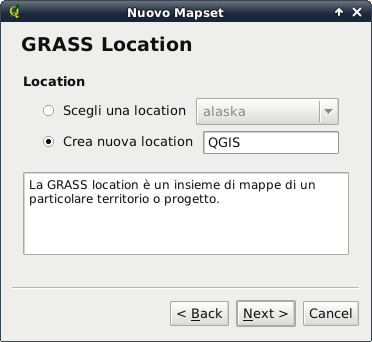
\includegraphics[clip=true, width=10cm]{create_grass_location}
\caption{Créer un nouveau SECTEUR ou JEU DE DONNEES \grass dans \qg \nixcaption}
\label{fig:create_grass_location}
\end{center}  
\end{figure}

\begin{enumerate}
  %\item Start \qg and make sure the \grass plugin is loaded
  \item Démarrez \qg et assurez vous que l'extension \grass est chargée.
  %\item Visualize the \filename{alaska.shp} Shapefile (see Section  \ref{sec:load_shapefile}) from the \qg alaska dataset~\ref{label_sampledata}.
  \item Affichez le shapefile \filename{alaska.shp} (voir Section \ref{sec:load_shapefile}) du jeu de données \qg Alaska ~\ref{label_sampledata}.
  %\item In the \grass toolbar, click on the \toolbtntwo{grass_open_mapset}{Open mapset} icon to bring up the \filename{MAPSET} wizard.
  \item Dans la barre d'outils \grass, cliquez sur \toolbtntwo{grass_new_mapset}{Nouveau jeu de données} pour ouvrir l'assistant \filename{Jeux de données}.
  % \item Select an existing \grass database (GISDBASE) folder \filename{grassdata} or create one for the new \filename{LOCATION} using a 
  % file manager on your computer. Then click \button{Next}.
  \item Sélectionnez un répertoire existant de base de données \grass (Base de données)\\ \filename {grassdata} ou créez en un pour le nouveau \filename{SECTEUR} avec le gestionnaire de fichiers de votre ordinateur. Cliquez le bouton \button{Suivant}.  
  % \item We can use this wizard to create a new \filename{MAPSET} within an 
  % existing \filename{LOCATION} (see Section~\ref{sec:add_mapset}) or to create 
  % a new \filename{LOCATION} altogether. Click on the radio button
  % \radiobuttonon{Create new location} (see Figure \ref{fig:create_grass_location}).
  \item Nous pouvons utiliser cet assistant à la fois pour créer un nouveau \filename{Jeu de données} dans un \filename{SECTEUR} existant (voir Section~\ref{sec:add_mapset}) et pour créer un nouveau \filename{SECTEUR}. Cliquez sur le bouton radio \radiobuttonon{Créez un nouveau secteur} (voir Figure \ref{fig:create_grass_location}).
  %\item Enter a name for the \filename{LOCATION} - we used Alaska and click \button{Next}
  \item Entrez un nom pour le \filename{SECTEUR} - nous utilisons Alaska et cliquez sur le bouton \button{Suivant}
  %\item Define the projection by clicking on the radio button \radiobuttonon{Projection} to enable the projection list 
  \item Définissez la projection en cliquant sur le bouton radio \radiobuttonon{Projection} pour activer la liste des projections
  % \item We are using Albers Equal Area Alaska (feet) projection. Since we happen to know that it is represented by the EPSG ID 2964, we enter it in
  % the search box. (Note: If you want to repeat this process for another \filename{LOCATION} and projection and haven't memorized the EPSG ID, 
  % click on the  \toolbtntwo{mIconProjectionEnabled}{projector} icon in the lower right-hand corner of the status bar (see Section \ref{label_projstart})).
  \item Nous utilisons la projection Albers Equal Area Alaska (pieds).Étant donné que nous savons qu'elle correspond au code EPSG 2964, nous le saisissons dans le champ de recherche. (Note : Si vous souhaitez reproduire la manipulation pour un autre \filename{SECTEUR} et une autre projection et que vous ne connaissez pas le code EPSG, cliquez sur\\ \toolbtntwo{mIconProjectionEnabled}{Statut de la projection} dans le coin inférieur droit de la barre d'état (voir Section \ref{label_projstart})).
  
  %\item Click \button{Find} to select the projection
  \item Cliquez sur \button{Trouver} pour sélectionner la projection
  %\item Click \button{Next} 
  \item Cliquer sur \button{Suivant}
  % \item To define the default region, we have to enter the \filename{LOCATION} 
  % bounds in north, south, east, and west direction. Here we simply click on 
  % the button \button{Set current \qg extent}, to apply the extend of the 
  % loaded layer \filename{alaska.shp} as the \grass default region extend.
  \item Pour définir la région par défaut, nous devons saisir les limites Nord, Sud , Est et Ouest du \filename{SECTEUR}. Ici il suffit de cliquer sur le bouton \button{Fixer l'emprise courante de \qg}, pour appliquer l'emprise du shapefile \filename{alaska.shp} déjà chargé comme emprise par défaut.
  %\item Click \button{Next}
  \item Cliquer sur \button{Suivant}
  % \item We also need to define a \filename{MAPSET} within our new \filename{LOCATION}. You can name it whatever you like - we used demo.
  % \footnote{When creating a new \filename{LOCATION}, \grass automatically 
  % creates a special \filename{MAPSET} called \filename{PERMANENT} designed to 
  % store the core data for the project, its default spatial extend and 
  % coordinate system definitions (Neteler \& Mitasova 2008 
  % \cite{neteler_mitasova08}).}
    \item Nous avons aussi besoin de définir un \filename{Jeu de données} dans notre nouveau \filename{SECTEUR}. Vous pouvez l'appeler comme vous le souhaitez - nous utiliserons demo. \footnote{Quand nous créons une nouveau \filename{SECTEUR}, \grass créé automatiquement un \filename{Jeu de données} spécial appelé \filename{PERMANENT} conçu pour stocker les données essentiels du projet, l'extension spatiale par défaut et la définition du système de coordonnées} (Neteler \& Mitasova 2008  \parencite{neteler_mitasova08}).
  % \item Check out the summary to make sure it's correct and click
  % \button{Finish}
  \item Vérifiez le résumé pour vous assurez que tout est correct et cliquez sur 
  \button{Terminer} 
  % \item The new \filename{LOCATION Alaska} and two \filename{MAPSETs demo}
  % and \filename{PERMANENT} are created. The currently opened working set is
  % \filename{MAPSET demo}, as you defined.
  \item Le nouveau \filename{SECTEUR Alaska} et les deux \filename{Jeux de données démo} et \filename{PERMANENT} sont créés. Actuellement, le jeu de données courant est le \filename{Jeux de données démo}, tel que vous l'avez défini.
  %\item Notice that some of the tools in the \grass toolbar that were disabled are now enabled.
  \item Notez que certains outils qui n'étaient pas accessibles le sont maintenant
\end{enumerate}

% If that seemed like a lot of steps, it's really not all that bad and a very 
% quick way to create a \filename{LOCATION}. The \filename{LOCATION alaska} is 
% now ready for data import (see Section \ref{sec:import_loc_data}).
% You can also use the already existing vector and raster data in the sample 
% \grass \filename{LOCATION alaska} included in the \qg alaska dataset 
% \ref{label_sampledata} and move on to Section \ref{label_vectmodel}.
Si cela semble faire beaucoup d'étapes, mais c'est en fait un moyen simple et rapide de créer un \filename{SECTEUR}. Le \filename{SECTEUR Alaska} est maintenant prêt pour l'importation de données (voir Section \ref{sec:import_loc_data}). Vous pouvez également utiliser des données raster ou vecteur existantes dans le \filename{SECTEUR Alaska} inclues dans le jeu de données \qg Alaska \ref{label_sampledata} et continuez dans la section \ref{label_vectmodel}.

%\subsection{Adding a new MAPSET}\label{sec:add_mapset}
\subsection{Ajouter un nouveau Jeu de données}\label{sec:add_mapset}

% A user has only write access to a \grass \filename{MAPSET} he created. This 
% means, besides access to his own \filename{MAPSET}, each user can also read 
% maps in other user's \filename{MAPSETs}, but he can modify or remove only 
% the maps in his own \filename{MAPSET}. All \filename{MAPSETs} include a 
% \filename{WIND} file that stores the current boundary coordinate values and 
% the currently selected raster resolution (Neteler \& Mitasova 2008 
% \cite{neteler_mitasova08}, see Section \ref{sec:grass_region}). 
Un utilisateur a seulement des droits d'écriture sur le \filename{Jeu de données} \grass qu'il a créé. Cela veut dire qu'au-delà de l'accès à son propre \filename{Jeu de données} \grass, chaque utilisateur peut aussi lire les données dans les autres \filename{Jeux de données}, mais il ne peut modifier et supprimer que les données que dans son propre \filename{Jeu de données}. Tous les \filename{Jeux de données} incluent un fichier \filename{WIND} qui stocke l'extension et la résolution raster courante (Neteler \& Mitasova 2008 \cite{neteler_mitasova08}, voir Section \ref{sec:grass_region}).

\begin{enumerate}
  %\item Start \qg and make sure the \grass plugin is loaded
  \item Démarrer \qg et assurez vous que l'extension \grass est chargée
  %\item In the \grass toolbar, click on the \toolbtntwo{grass_new_mapset}{New mapset} icon to bring up the  \filename{MAPSET} wizard.
  \item Dans la barre d'outils \grass, cliquez sur \toolbtntwo{grass_new_mapset}{Nouveau jeu de données} pour ouvrir l'assistant \filename{Jeux de données}.
  %\item Select the \grass database (GISDBASE) folder \filename{grassdata} with the \filename{LOCATION alaska}, where we want to add a further 
  %\filename{MAPSET}, called test.
  \item Sélectionnez le répertoire \filename{grassdata} de la base de données \grass (Base de données) qui contient déjà le \filename{SECTEUR Alaska} et où nous voulons ajouter un autre \filename{SECTEUR} nommé test.
  %\item Click \button{Next}.
  \item Cliquez sur \button{Suivant}. 
  %\item We can use this wizard to create a new \filename{MAPSET} within an existing \filename{LOCATION} or to create a new \filename{LOCATION} 
  %altogether. Click on the radio button \radiobuttonon{Select location} (see Figure \ref{fig:create_grass_location}) and click \button{Next}.
  \item Nous pouvons utiliser cet assistant à la fois pour créer un nouveau \filename{Jeu de données} dans le \filename{SECTEUR} existant et pour créer un nouveau \filename{SECTEUR}. Cliquez sur le bouton radio\\ \radiobuttonon{Sélectionnez le Secteur} (voir Figure \ref{fig:create_grass_location}) et cliquez sur \button{Suivant}.
  %\item Enter the name \filename{text} for the new \filename{MAPSET}. Below in the wizard you see a list of existing \filename{MAPSETs} and its owners.
  \item Entrez le \filename{text} du nom pour le nouveau \filename{Jeu de données}. En dessous, dans l'assistant, vous pouvez voir une liste des \filename{Jeux de données} et de leurs propriétaires.
  %\item Click \button{Next}, check out the summary to make sure it's all correct and click \button{Finish}
  \item Cliquez sur \button{Suivant}, vérifiez le résumé pour vous assurer qu'il est correct et cliquez sur \button{Terminer}
\end{enumerate}

%\section{Importing data into a \grass LOCATION}\label{sec:import_loc_data}
\section{Importer des données dans un SECTEUR \grass}\label{sec:import_loc_data}

% This Section gives an example how to import raster and vector data into the 
% \filename{alaska} \grass \filename{LOCATION} provided by the \qg alaska 
% dataset. Therefore we use a landcover raster map \filename{landcover.img} 
% and a vector GML File \filename{lakes.gml} from the \qg alaska 
% dataset \ref{label_sampledata}.
Cette section donne un exemple d'importation de données raster et vecteur dans le \filename{SECTEUR} \grass \filename{Alaska} fournit dans le jeu de données \qg Alaska. Nous utiliserons une couche raster d'occupation du sol \filename{landcover.img} et une couche vecteur au format GML \filename{lakes.gml}, toutes deux présentes dans le jeu de données Alaska.

\begin{enumerate}
  %\item Start \qg and make sure the \grass plugin is loaded.
  \item Démarrer \qg et assurez vous que l'extension \grass est chargée.
  %\item In the \grass toolbar, click the \toolbtntwo{grass_open_mapset}{Open MAPSET} icon to bring up the \filename{MAPSET} wizard.
  \item Dans la barre d'outils \grass, cliquez sur \toolbtntwo{grass_open_mapset}{Ouvrir un jeu de données} pour ouvrir l'assistant \filename{Jeu de données}.
  %\item Select as \grass database the folder \filename{grassdata} in the \qg alaska dataset, as \filename{LOCATION alaska}, as \filename{MAPSET} 
  %\filename{demo} and click \button{OK}.
  \item Sélectionnez comme base de données \grass le répertoire \filename{grassdata} dans le jeu de données \qg Alaska, comme \filename{SECTEUR Alaska}, comme as \filename{Jeu de donnée} \filename{démo} et cliquez sur \button{OK}.
  %\item Now click the \toolbtntwo{grass_tools}{Open \grass tools} icon. The \grass Toolbox (see Section \ref{subsec:grass_toolbox}) dialog appears.
  \item Maintenant cliquez sur \toolbtntwo{grass_tools}{Ouvrir les outils \grass}. La boîte à outils \grass (voir Section \ref{subsec:grass_toolbox}) s'ouvre.
  %\item To import the raster map \filename{landcover.img}, click the module \filename{r.in.gdal} in the \tab{Modules Tree} tab. This \grass module allows to import GDAL supported raster files into a \grass \filename{LOCATION}. The module dialog for \filename{r.in.gdal} appears.
  \item  Pour importer la couche raster \filename{landcover.img}, cliquez sur le module \filename{r.in.gdal} dans l'onglet \tab{Arborescence des modules}. Ce module \grass vous permet d'importer les fichiers raster supportés par la librairie GDAL dans un \filename{SECTEUR} \grass. La boîte de dialogue  \filename{r.in.gdal} apparaît.
  %\item Browse to the folder \filename{raster} in the \qg alaska dataset and select the file \filename{landcover.img}.
  \item Naviguer jusqu'au répertoire \filename{raster} dans le jeu de données \qg Alaska et sélectionnez le fichier \filename{landcover.img}.
  %\item As raster output name define \filename{landcover\_grass} and click \button{Lancer}. In the \tab{Output} tab you see the currently running \grass command \filename{r.in.gdal -o input=/path/to/landcover.img output=landcover\_grass}.
  \item Définissez \filename{landcover\_grass} comme nom de sortie et cliquez sur \button{Lancer}. Dans l'onglet \tab{Rendu}, vous voyez la commande \grass en cours\\ \filename{r.in.gdal -o input=/path/to/landcover.img output=landcover\_grass}.
  %\item When it says \textbf{Succesfully finished} click \button{Vue}. 
  \item Lorsque \textbf{Terminé avec succès} s'affiche cliquez sur \button{Vue}. 
  %The \filename{landcover\_grass} raster layer is now imported into \grass and will be visualized in the \qg canvas.
  La couche raster\\ \filename{landcover\_grass} est maintenant importée dans \grass et pourra être affichée dans \qg.
  
  %\item To import the vector GML file \filename{lakes.gml}, click the module \filename{v.in.ogr} in the \tab{Modules Tree} tab. This \grass module allows to import OGR supported vector files into a \grass \filename{LOCATION}. The module dialog for \filename{v.in.ogr} appears.
  \item Pour importer le fichier GML \filename{lakes.gml}, cliquez sur le module \filename{v.in.ogr} dans l'onglet \tab{Arborescence des modules}.La boîte de dialogue  \filename{v.in.ogr} apparaît.
  %\item Browse to the folder \filename{gml} in the \qg alaska dataset and select the file \filename{lakes.gml} as OGR file.
  \item Naviguer jusqu'au répertoire \filename{gml} dans le jeu de données \qg Alaska et sélectionnez le fichier \filename{lakes.gml}.
  %\item As vector output name define \filename{lakes\_grass} and click \button{Lancer}. You don't have to care about the other options in this   example. In the \tab{Output} tab you see the currently running \grass command \filename{v.in.ogr -o dsn=/path/to/lakes.gml output=lakes\_grass}.
  \item Définissez \filename{lakes\_grass} comme nom de sortie et cliquez sur \button{Lancer}. Vous n'avez pas besoin des autres options dans cet exemple.
  %\item When it says \textbf{Succesfully finished} click \button{Vue}. 
  \item Lorsque \textbf{Terminé avec succès} s'affiche cliquez sur \button{Vue}. 
  %The \filename{lakes\_grass} vector layer is now imported into \grass and will be visualized in the \qg canvas. 
  Le fichier \filename{lakes\_grass} est maintenant importé dans \grass et pourra être affiché dans \qg.
 
\end{enumerate}


%\section{The \grass vector data model}\label{label_vectmodel}\index{\grass!vector data model}
\section{Le modèle vecteur de \grass}\label{label_vectmodel}\index{\grass!modèle vecteur}

% It is important to understand the \grass vector data model prior to
% digitizing.\index{\grass!digitizing} In general, \grass uses a topological
% vector model.\index{\grass!topology} This means that areas are not represented
% as closed polygons, but by one or more boundaries. A boundary between two
% adjacent areas is digitized only once, and it is shared by both areas.
% Boundaries must be connected without gaps. An area is identified (labeled) 
% by the centroid of the area.
Il est important de comprendre le modèle vecteur de \grass avant de faire de la numérisation.\index{\grass!numérisation} En général, \grass utilise un modèle vecteur topologique.\index{\grass!topologie} Cela veut dire que les surfaces ne sont pas représentées par des polygones fermés, mais par une ou plusieurs limites. Une limite entre des polygones adjacents n'est numérisée qu'une seule fois et est partagée par les deux surfaces. Les limites doivent être connectées sans trous. Une surface est identifiée (libellée) via le centroide de la surface.

% Besides boundaries and centroids, a vector map can also contain
% points and lines. All these geometry elements can be mixed
% in one vector and will be represented in different so called 'layers' inside
% one \grass vector map. So in \grass a layer is not a vector or raster map but a
% level inside a vector layer. This is important to distinguish carefully.
% \footnote{Although it is possible to mix geometry elements, it is unusual and even in \grass only
% used in special cases such as vector network analysis. Normally you should
% prefere to store different geometry elements in different layers.}

Outre les limites et centroïdes, une couche vecteur peut également contenir des points et des lignes. Tous ces éléments de géométrie peuvent être mélangés dans une couche vecteur et seront représentés dans différentes «sous-couches» dans une carte vectorielle \grass. Ainsi, une couche \grass n'est pas un vecteur ou un raster, mais un niveau à l'intérieur d'une couche vecteur. Il est important de bien distinguer ceci.
\footnote{Même s'il est possible de mélanger des éléments de géométries différentes, c'est inhabituel et même dans \grass, on l'utilise dans des cas particuliers tel que l'analyse de réseau. Normalement, vous devriez stocker des éléments de géométries différentes dans des couches différentes}

% It is possible to store more 'layers' in one vector dataset. For example,
% fields, forests and lakes can be stored in one vector. Adjacent
% forest and lake can share the same boundary, but they have separate attribute
% tables. It is also possible to attach attributes to boundaries. For example,
% the boundary between lake and forest is a road, so it can have a different 
% attribute table.

Il est possible de stocker plusieurs sous-couches dans une couche vecteur. Par exemple, des champs, de la forêt et des lacs peuvent être stockés dans une couche vecteur. Les forêts et les lacs adjacents partagent les mêmes limites, mais ils auront des tables attributaires différentes. Il est aussi possible de faire correspondre une table attributaire aux limites. Par exemple, la limite entre un lac et une forêt peut être une route qui peut avoir une table attributaire différente.

% The 'layer' of the feature is defined by 'layer' inside \grass. 'Layer' is the 
% number which defines if there are more than one layer inside the dataset, e.g. 
% if the geometry is forest or lake. For now, it can be only a number, in the 
% future \grass will also support names as fields in the user interface.

La \og sous-couche\fg est définie dans \grass par un chiffre. Ce chiffre définit s'il y a plusieurs sous-couches à l'intérieur d'une couche vecteur. Par exemple, il définit s'il s'agit de lac ou de forêt. Pour l'instant, il s'agit d'un nombre, mais dans des versions futures \grass pourra utiliser des noms pour les sous-couches dans l'interface utilisateur.

% Attributes can be stored inside the \grass \filename{LOCATION} as DBase or 
% SQLITE3 or in external database tables, for example PostgreSQL, MySQL,Oracle, etc.\index{\grass!attribute storage}
Les données attributaires peuvent être stockées dans le \filename{SECTEUR} au format DBase ou SQLIte3 ou dans des tables de bases de données externes comme par exemple : PostgreSQL, MySQL, Oracle, etc.\index{\grass!stockage des attributs}

% Attributes in database tables are linked to geometry elements using
% a 'category' value.\index{\grass!attribute linkage} 'Category' (key, ID) is an
% integer attached to geometry primitives, and it is used as the link to one
% key column in the database table.

Les données attributaires sont liées à la géométrie par le biais d'un champ \og category\fg.\index{\grass!liens des attributs} \og Category\fg (clé, ID) est un entier attaché à la géométrie, et il est utilisé comme lien vers une colonne de clé dans la table de base de données.

%\begin{Tip}\caption{\textsc{Learning the \grass Vector Model}}
\begin{Tip}\caption{\textsc{Apprendre le modèle vecteur de \grass}}
%The best way to learn the \grass vector model and its capabilities is to download one of the many \grass tutorials where the vector model is described
%more deeply. See \url{http://grass.osgeo.org/gdp/manuals.php} for more information, books and tutorials in several languages.
Le meilleur moyen d'apprendre le modèle vecteur de \grass et ses possibilités est de télécharger un des nombreux tutoriels \grass où le modèle vecteur est décrit plus précisément. Voir \url{http://grass.osgeo.org/gdp/manuals.php} pour des informations complémentaires, des livres et des tutoriels dans différentes langues.
\end{Tip} 

%\section{Creating a new \grass vector layer}\label{sec:creating_new_grass_vectors}\index{\grass!Creating new vectors|see{editing!creating a new layer}}
\section{Création d'une nouvelle couche vecteur \grass}\label{sec:creating_new_grass_vectors}\index{\grass!Créer de nouvelles couches vecteur|voir{éditer!créer une nouvelle couche}}

% To create a new \grass vector layer with the \grass plugin click the 
% \toolbtntwo{grass_new_vector_layer}{Create new \grass vector} toolbar icon. 
% Enter a name in the text box and you can start digitizing point, line or 
% polygone geometries, following the procedure described in Section 
% \ref{grass_digitising}. 
Pour créer une nouvelle couche vecteur \grass à l'aide de l'extension \grass, cliquez sur \toolbtntwo{grass_new_vector_layer}{Créez une nouvelle couche vectorielle \grass} dans la barre d'outils. Entrez le nom dans la boîte de dialogue et vous pouvez commencer à digitaliser un point une ligne ou un polygone en suivant les instructions de la section \ref{grass_digitising}.

% In \grass it is possible to organize all sort of geometry types (point, line 
% and area) in one layer, because \grass uses a topological vector model, so you 
% don't need to select the geometry type when creating a new \grass vector. This 
% is different from Shapefile creation with \qg, because Shapefiles use the 
% Simple Feature vector model (see Section \ref{sec:create shape}).
Dans \grass, il est possible de gérer plusieurs types de géométrie (point, ligne et surface) dans une seule couche d'information, car \grass utilise un modèle vecteur topologique. Vous n'avez donc pas besoin de sélectionner un type de géométrie quand vous créez une couche vecteur \grass. C'est différent de la création de shapefile avec \qg, car les shapefiles utilisent un modèle vecteur d'entité simple (Simple Feature vector model) (voir Section \ref{sec:create shape}).

%\begin{Tip}\caption{\textsc{Creating an attribute table for a new \grass vector layer}}
\begin{Tip}\caption{\textsc{Création d'une table attributaire pour une nouvelle couche vecteur \grass}}
% If you want to assign attributes to your digitized geometry features, make sure to create an attribute table with columns before you start digitizing (see Figure \ref{fig:grass_digitizing_table}).
Si vous souhaitez renseigner les données attributaires de vos entités numérisées, assurez-vous d'avoir créé une table attributaire avec des champs avant ce commencer votre numérisation (voir Figure \ref{fig:grass_digitizing_table}).
%\end{Tip} 
\end{Tip}

%\section{Digitizing and editing a \grass vector layer}\index{\grass!digitizing tools}\label{grass_digitising}
\section{Numérisation et édition de couche vecteur \grass}\index{\grass!outils de numérisation}\label{grass_digitising}

% The digitizing tools for \grass vector layers are accessed using the
% \toolbtntwo{grass_edit}{Edit \grass vector layer} icon on the toolbar. Make 
% sure you have loaded a \grass vector and it is the selected layer in the legend 
% before clicking on the edit tool. Figure \ref{fig:grass_digitizing_category} 
% shows the \grass edit dialog that is displayed when you click on the edit tool. 
% The tools and settings are discussed in the following sections.
Les outils de numérisation pour les couches vecteurs de \grass sont accessibles via\\ \toolbtntwo{grass_edit}{Éditer une couche vectorielle \grass} dans la barre d'outils. Assurez-vous d'avoir ouvert une couche vectorielle \grass ainsi que d'avoir sélectionné la sous-couche dans la légende avant d'utiliser l'outil d'édition. La figure \ref{fig:grass_digitizing_category} montre la boîte de dialogue \grass qui s'affiche quand vous cliquez sur l'outil d'édition. Les outils et les paramètres d'édition sont détaillés dans les paragraphes suivants.

%\begin{Tip}\caption{\textsc{Digitizing polygones in \grass}}
\begin{Tip}\caption{\textsc{Numérisation de polygones dans \grass}}
% If you want to create a polygone in \grass, you first digitize the boundary of 
% the polygon, setting the mode to \usertext{No category}. Then you add a 
% centroid (label point) into the closed boundary, setting the mode to 
% \usertext{Next not used}. The reason is, that a topological vector model links 
% attribute information of a polygon always to the centroid and not to the 
% boundary.
% }
Si vous voulez créer un polygone dans \grass, vous devez numériser premièrement les limites du polygone, en définissant mode sur \usertext{Pas de catégorie}.Ensuite, vous ajoutez un centroïde (emplacement de l'étiquette) dans le polygone fermé, fixant le mode sur \usertext{Prochain non utilisé}. La raison en est, que le modèle vectoriel topologique assure toujours le lien entre les informations d'attributs des polygones via le centroïde et non via la limite.
\end{Tip}
%\end{Tip} 

%\minisec{Toolbar}\label{label_grasstoolbar}
\minisec{Barre d'outils}\label{label_grasstoolbar}

% In Figure \ref{fig:grass_digitizing_toolbar} you see the \grass digitizing
% toolbar icons provided by the \grass plugin. Table \ref{tab:grass_tools}
% explains the available functionalities.
Sur la figure \ref{fig:grass_digitizing_toolbar} vous pouvez voir la barre d'outils d'édition \grass de l'extension \grass. Le tableau \ref{tab:grass_tools} récapitule les fonctions disponibles.

\begin{figure}[h]
   \begin{center}
   %\caption{\grass Digitizing Toolbar \nixcaption}\label{fig:grass_digitizing_toolbar}
   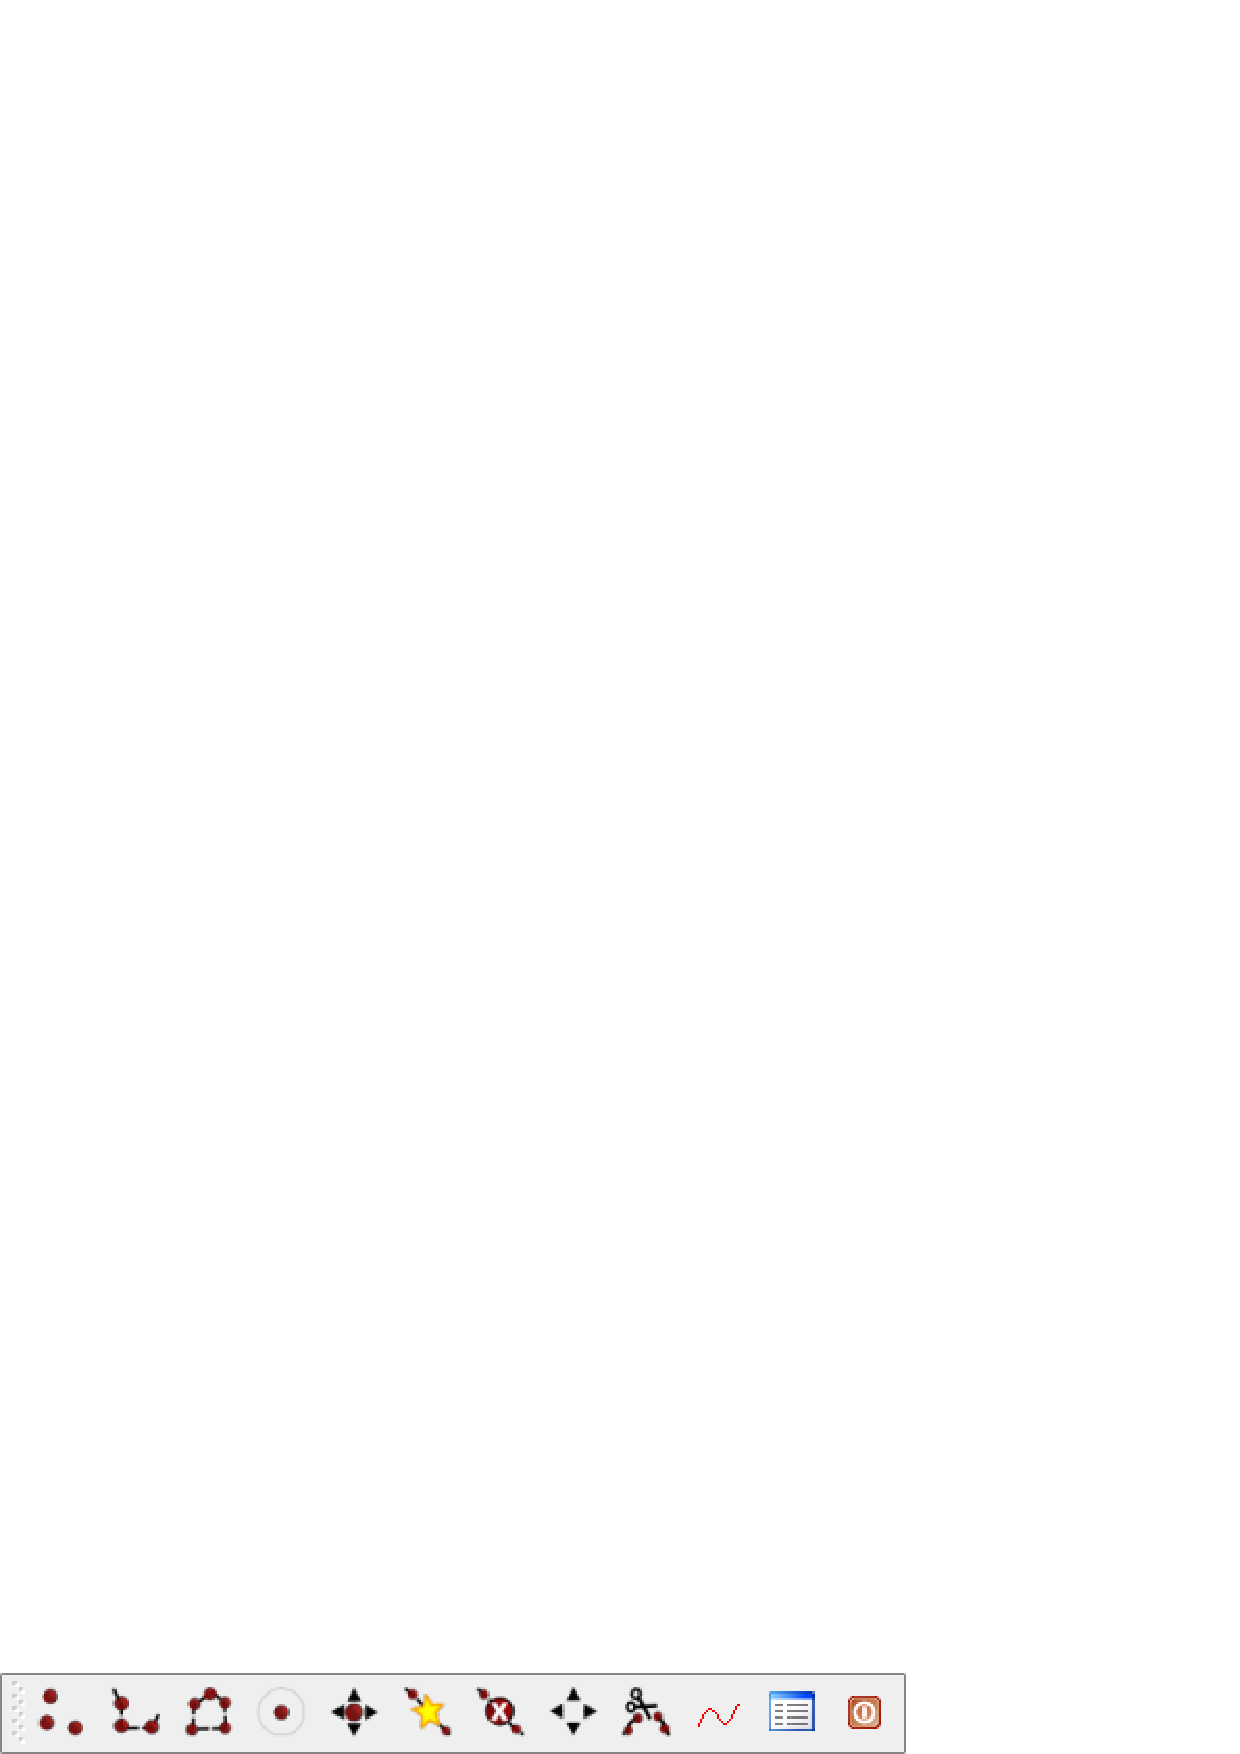
\includegraphics[clip=true,width=12cm]{grass_digitizing_toolbar}
   \caption{Barre d'outils d'édition \grass \nixcaption}\label{fig:grass_digitizing_toolbar} 
\end{center}  
\end{figure}
{\renewcommand{\arraystretch}{2}
\begin{table}[p]\index{\grass!digitizing tools}
\centering
 \begin{tabular}{|m{1cm}|m{4cm}|m{8.5cm}|}
% \hline \textbf{Icon} & \textbf{Tool} & \textbf{Purpose} \\
% \hline 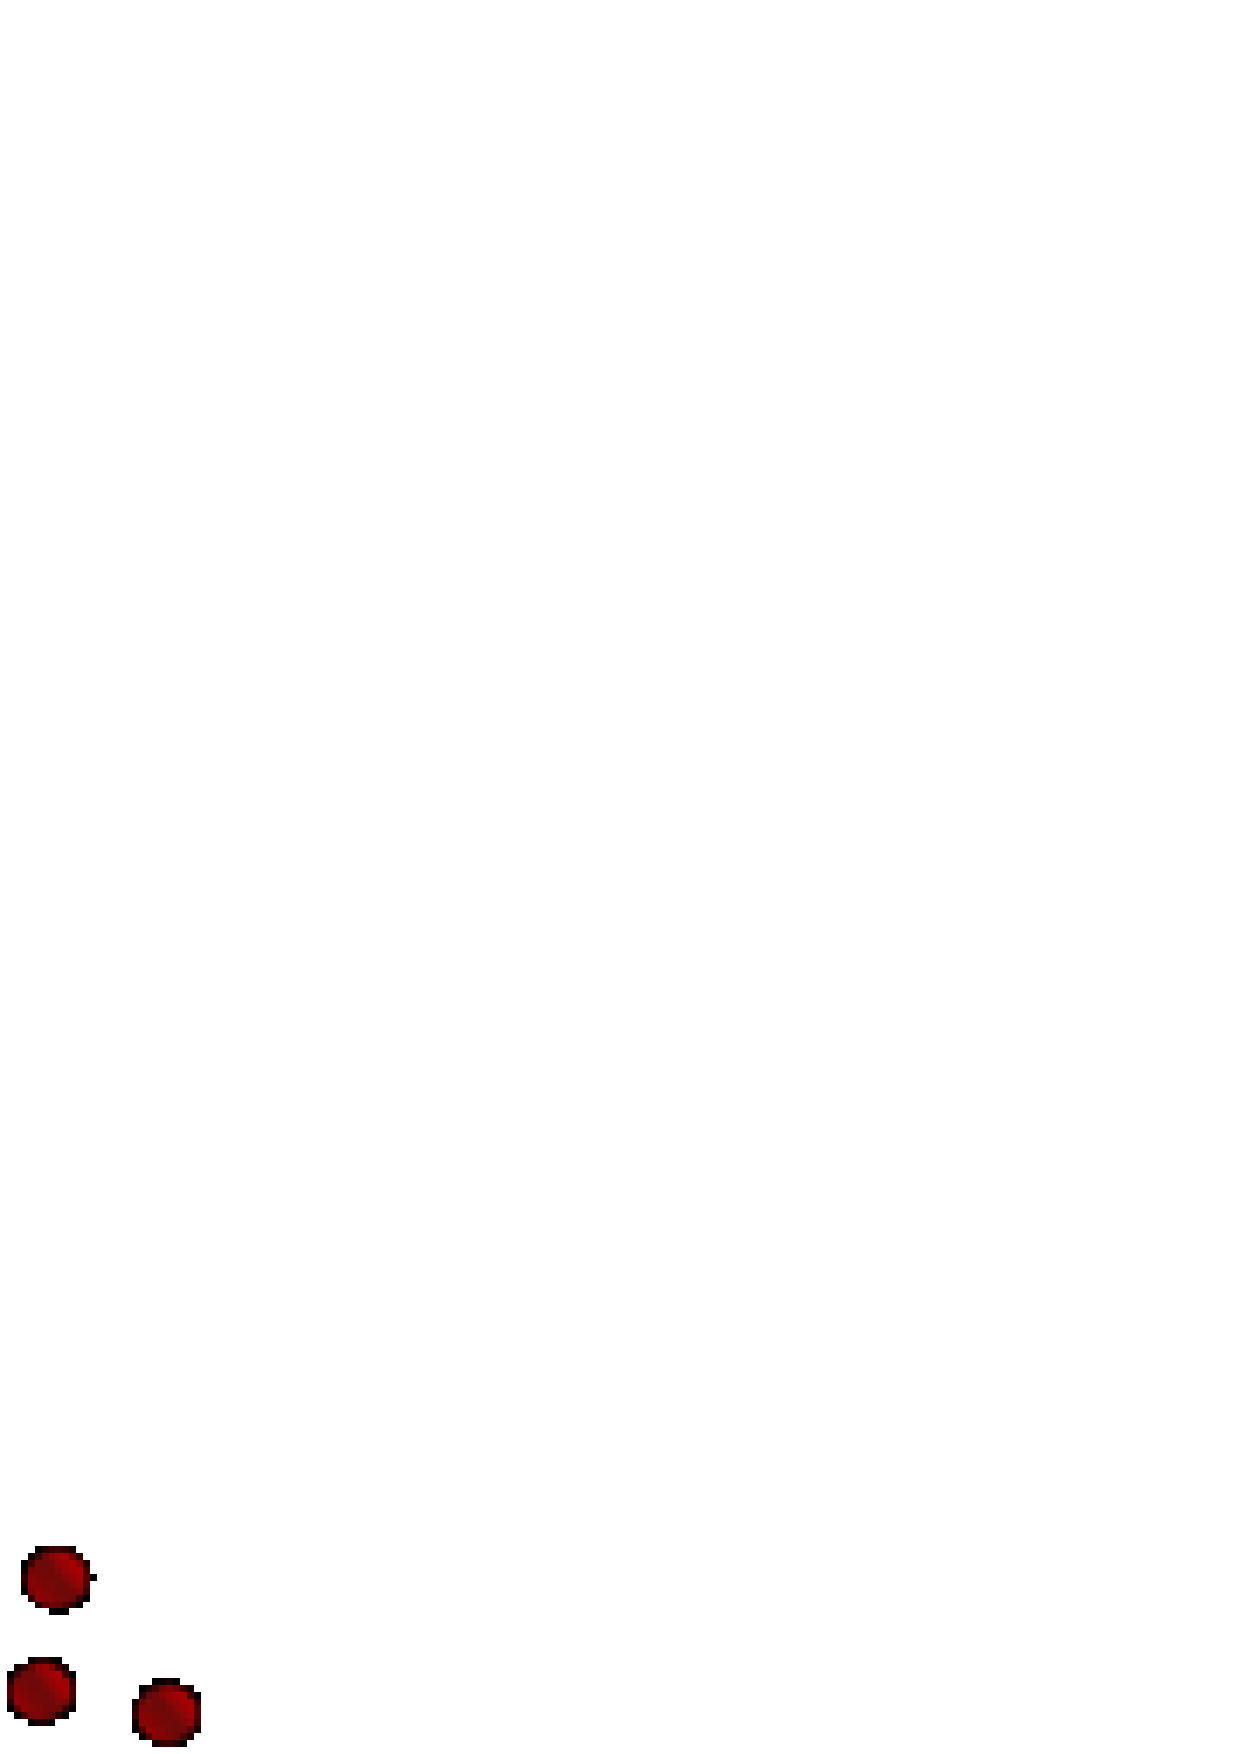
\includegraphics[width=0.7cm]{grass_new_point} & New Point & Digitize
% new point \\
% \hline 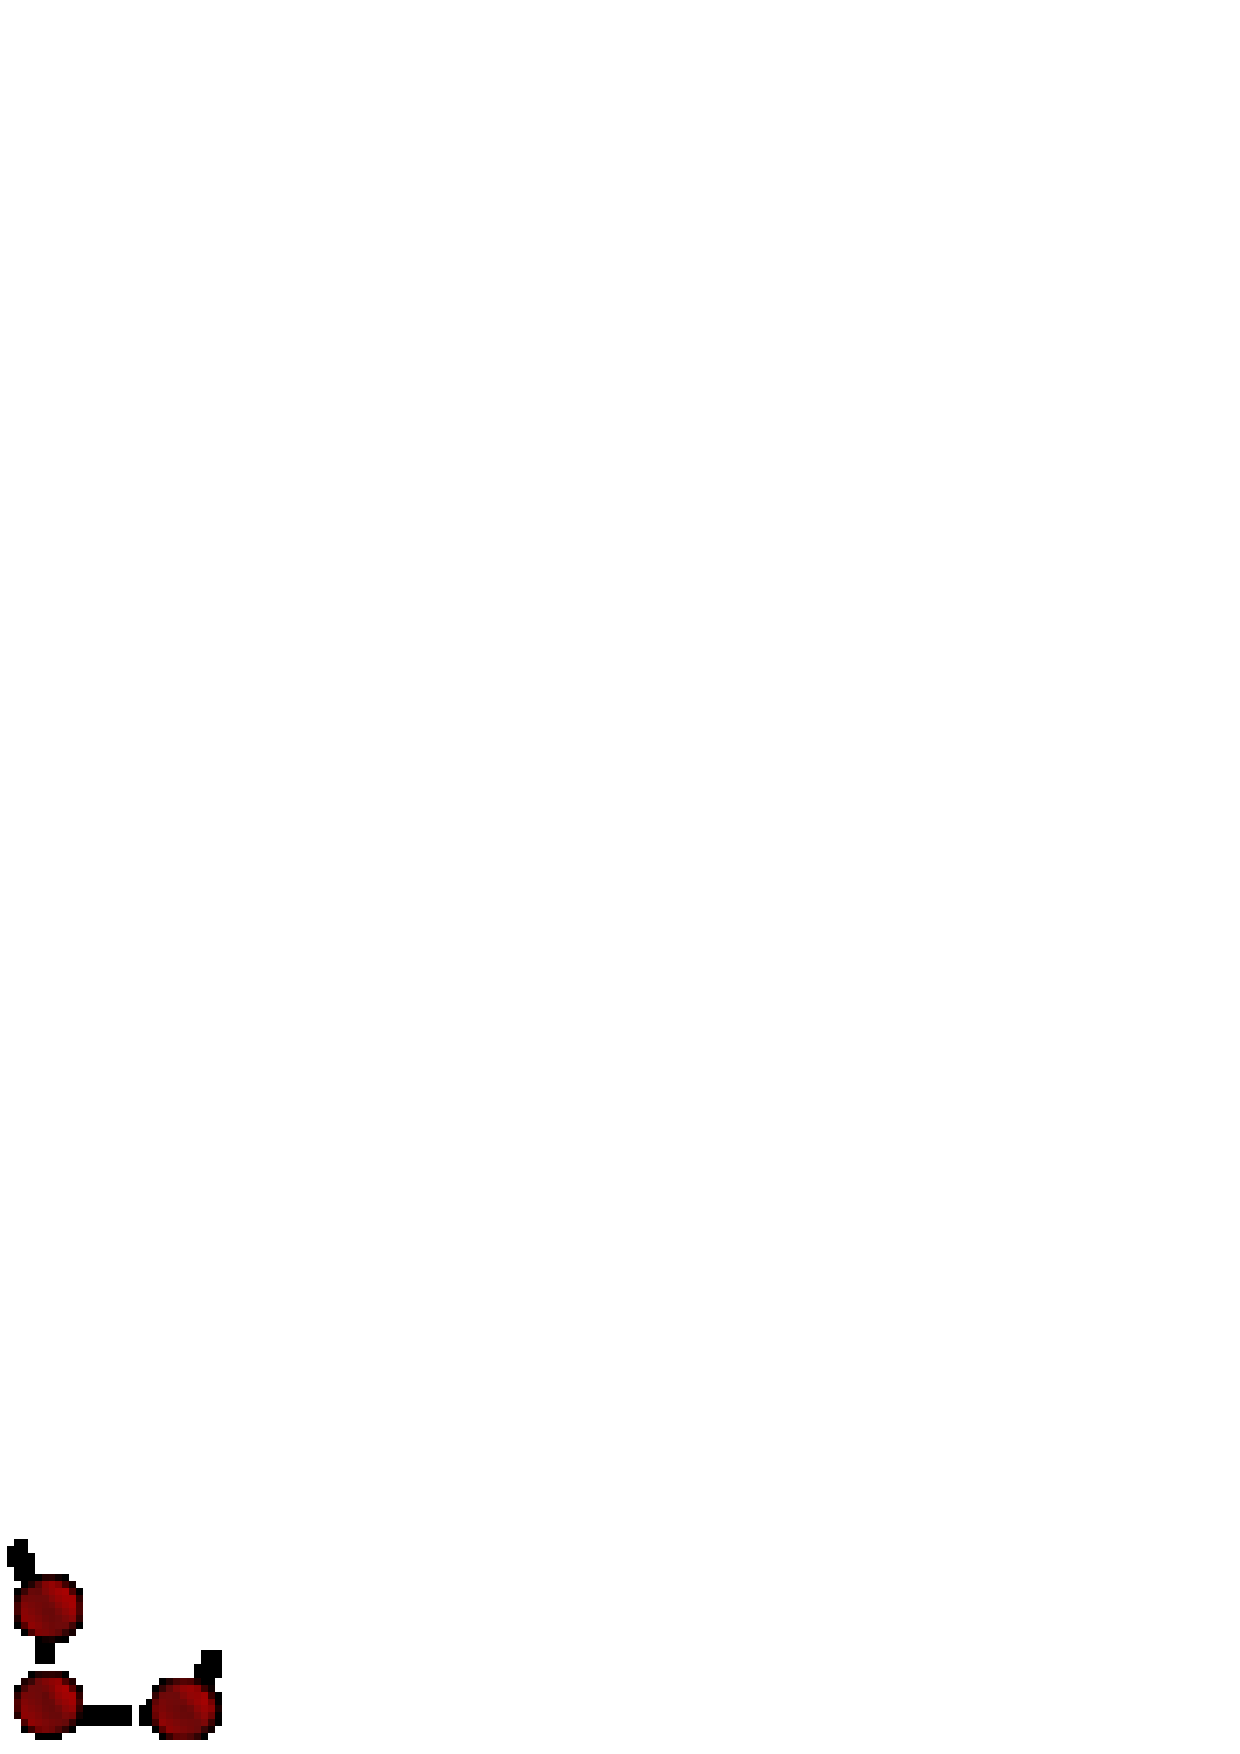
\includegraphics[width=0.7cm]{grass_new_line} & New Line & Digitize
% new line (finish by selecting new tool) \\
% \hline 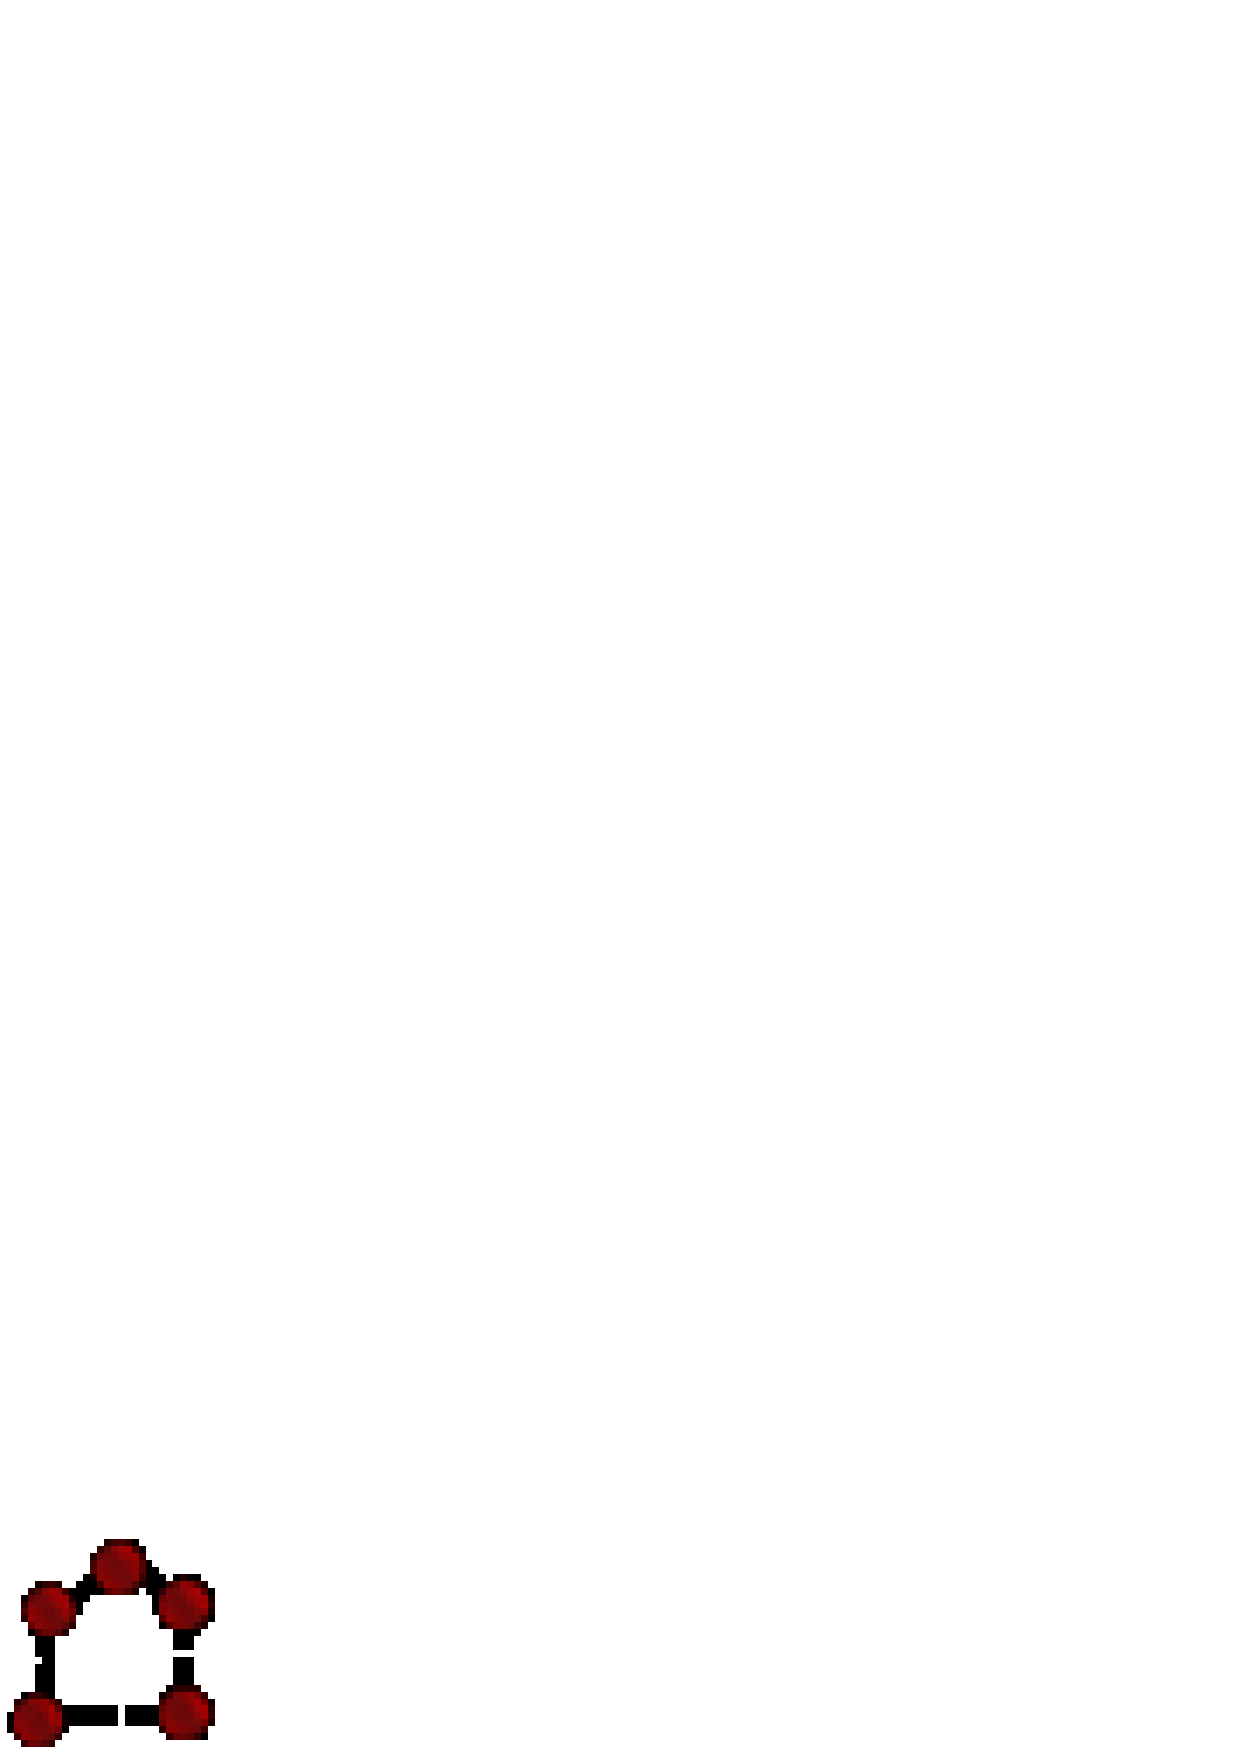
\includegraphics[width=0.7cm]{grass_new_boundary} & New Boundary &
% Digitize new boundary (finish by selecting new tool)\\
% \hline 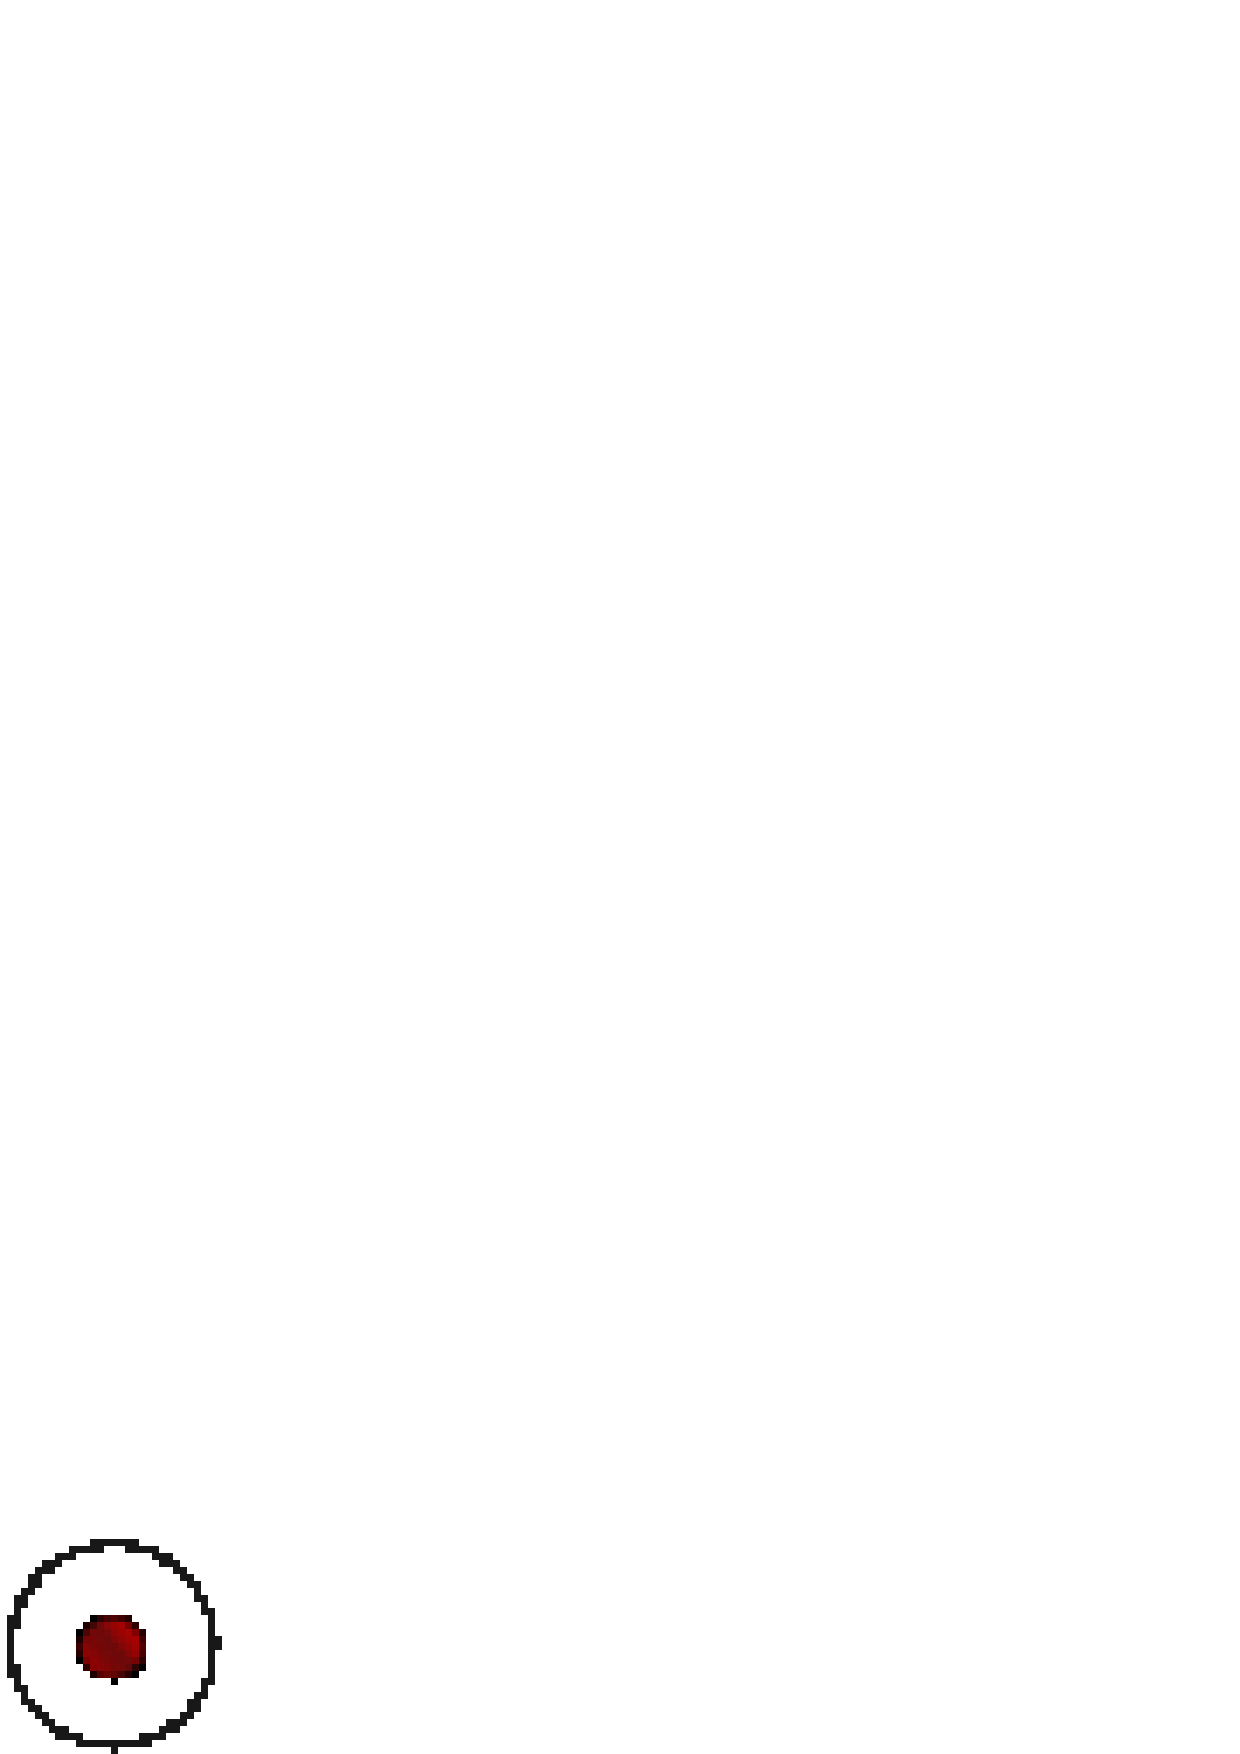
\includegraphics[width=0.7cm]{grass_new_centroid} & New Centroid &
% Digitize new centroid (label existing area)\\
% \hline 
\includegraphics[width=0.7cm]{grass_move_vertex} & Move vertex & Move
% one vertex of existing line or boundary and identify new position\\
% \hline 
\includegraphics[width=0.7cm]{grass_add_vertex} & Add vertex & Add a
% new vertex to existing line\\
% \hline 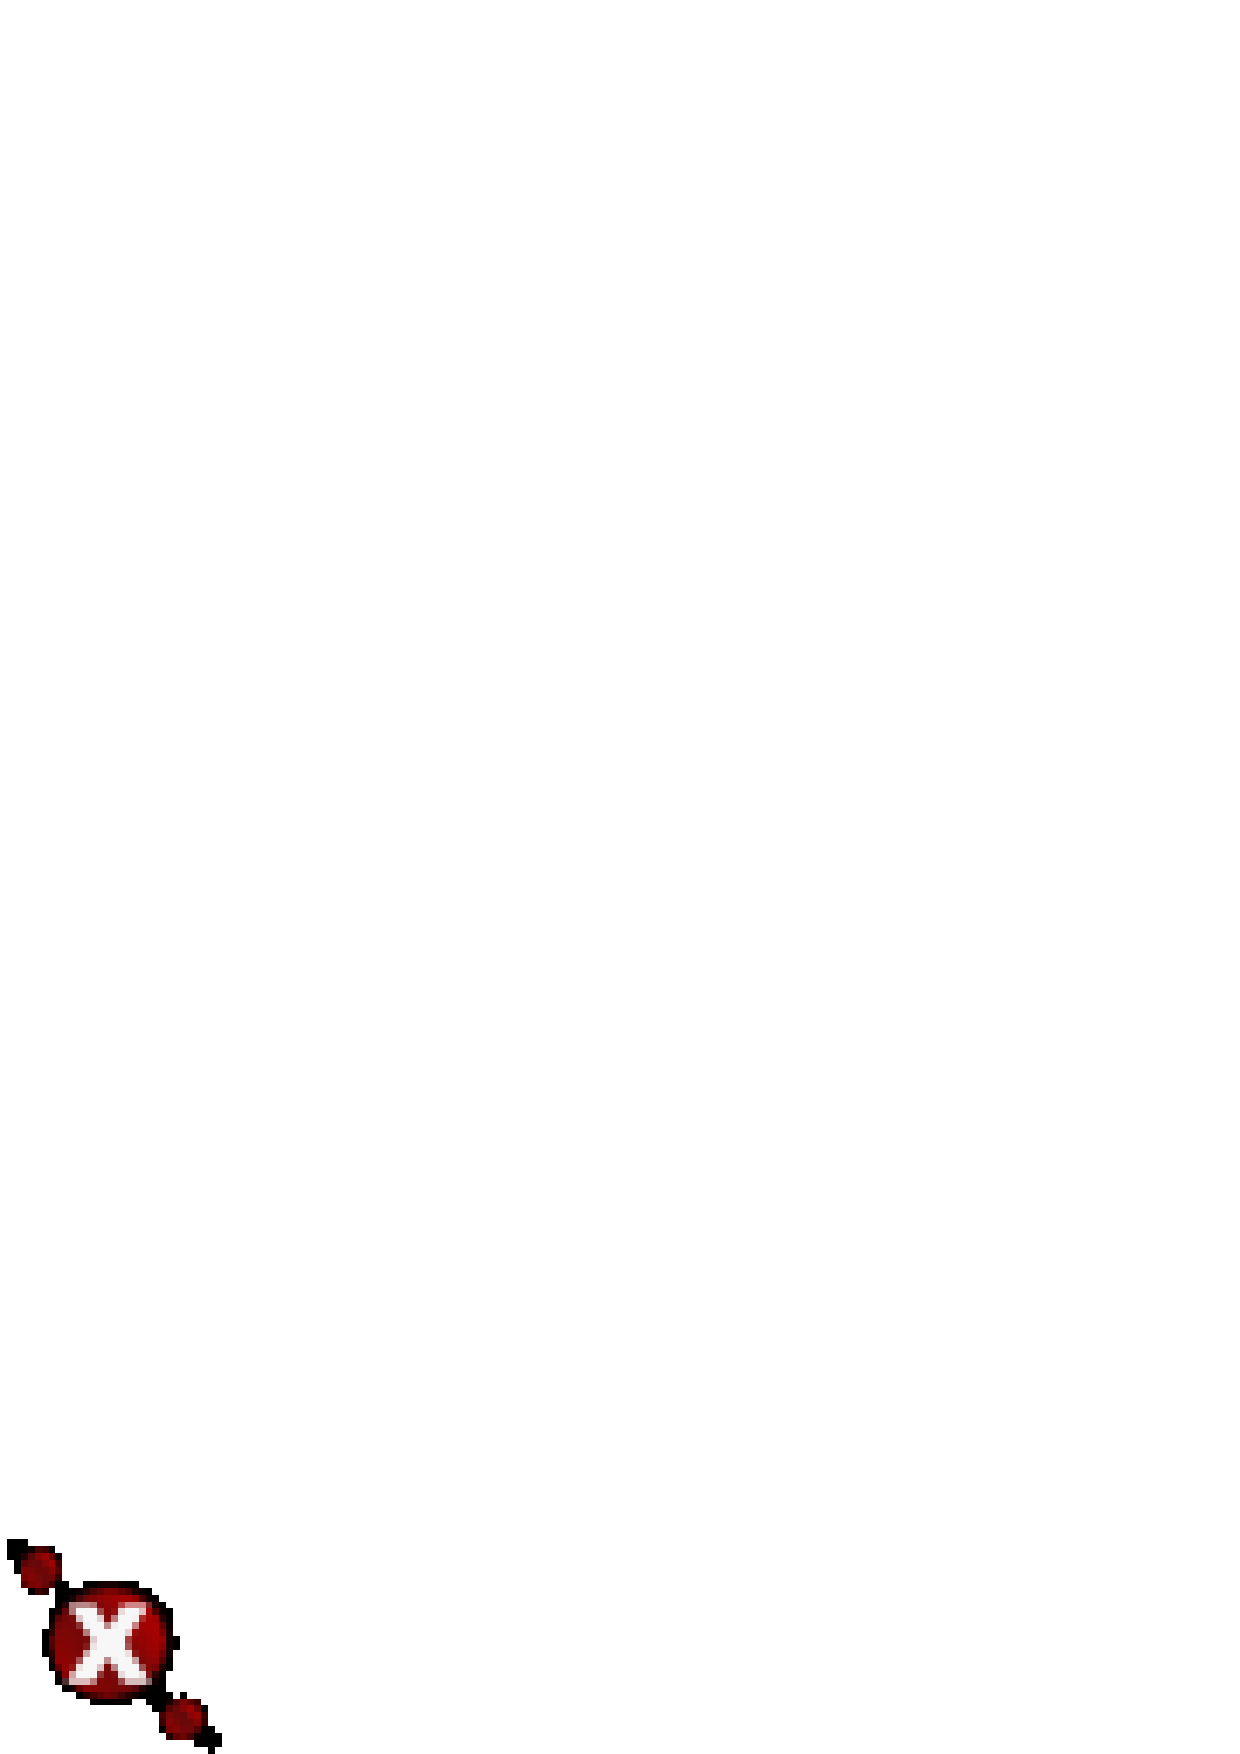
\includegraphics[width=0.7cm]{grass_delete_vertex} & Delete vertex &
% Delete vertex from existing line (confirm selected vertex by another click)\\
% \hline 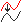
\includegraphics[width=0.7cm]{grass_move_line} & Move element & Move
% selected boundary, line, point or centroid and click on new position\\
% \hline 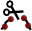
\includegraphics[width=0.7cm]{grass_split_line} & Split line & Split
% an existing line to 2 parts\\
% \hline 
\includegraphics[width=0.7cm]{grass_delete_line} & Delete element &
% Delete existing boundary, line, point or centroid (confirm selected element by
% another click)\\
% \hline 
\includegraphics[width=0.7cm]{grass_edit_attributes} & Edit attributes
% & Edit attributes of selected element (note that one element can represent
% more features, see above)\\
% \hline 
\includegraphics[width=0.7cm]{grass_close_edit} & Close & Close
% session and save current status (rebuilds topology afterwards)\\
% \hline
\hline \textbf{Icône} & \textbf{Outil} & \textbf{Fonction} \\
\hline 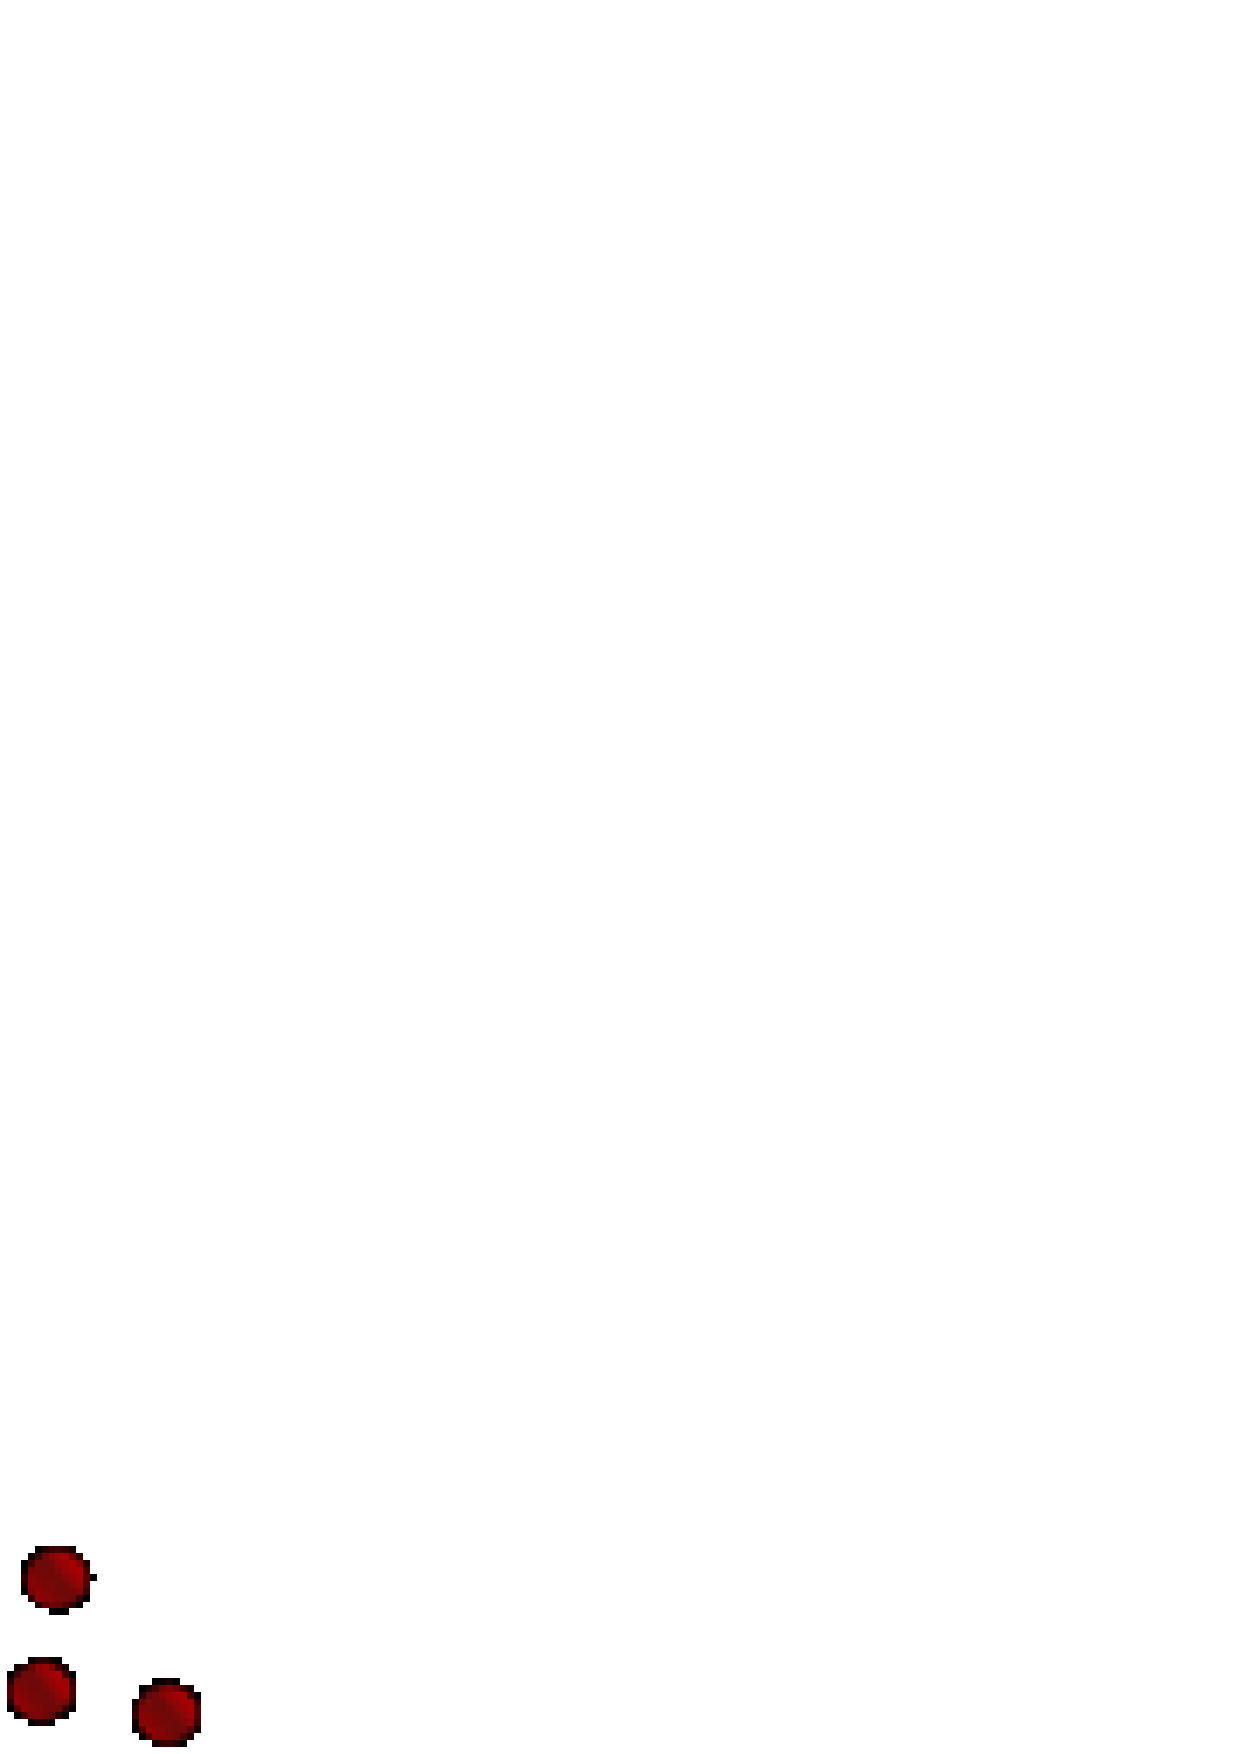
\includegraphics[width=0.7cm]{grass_new_point} & Nouveau Point & Numérise un nouveau point \\
\hline 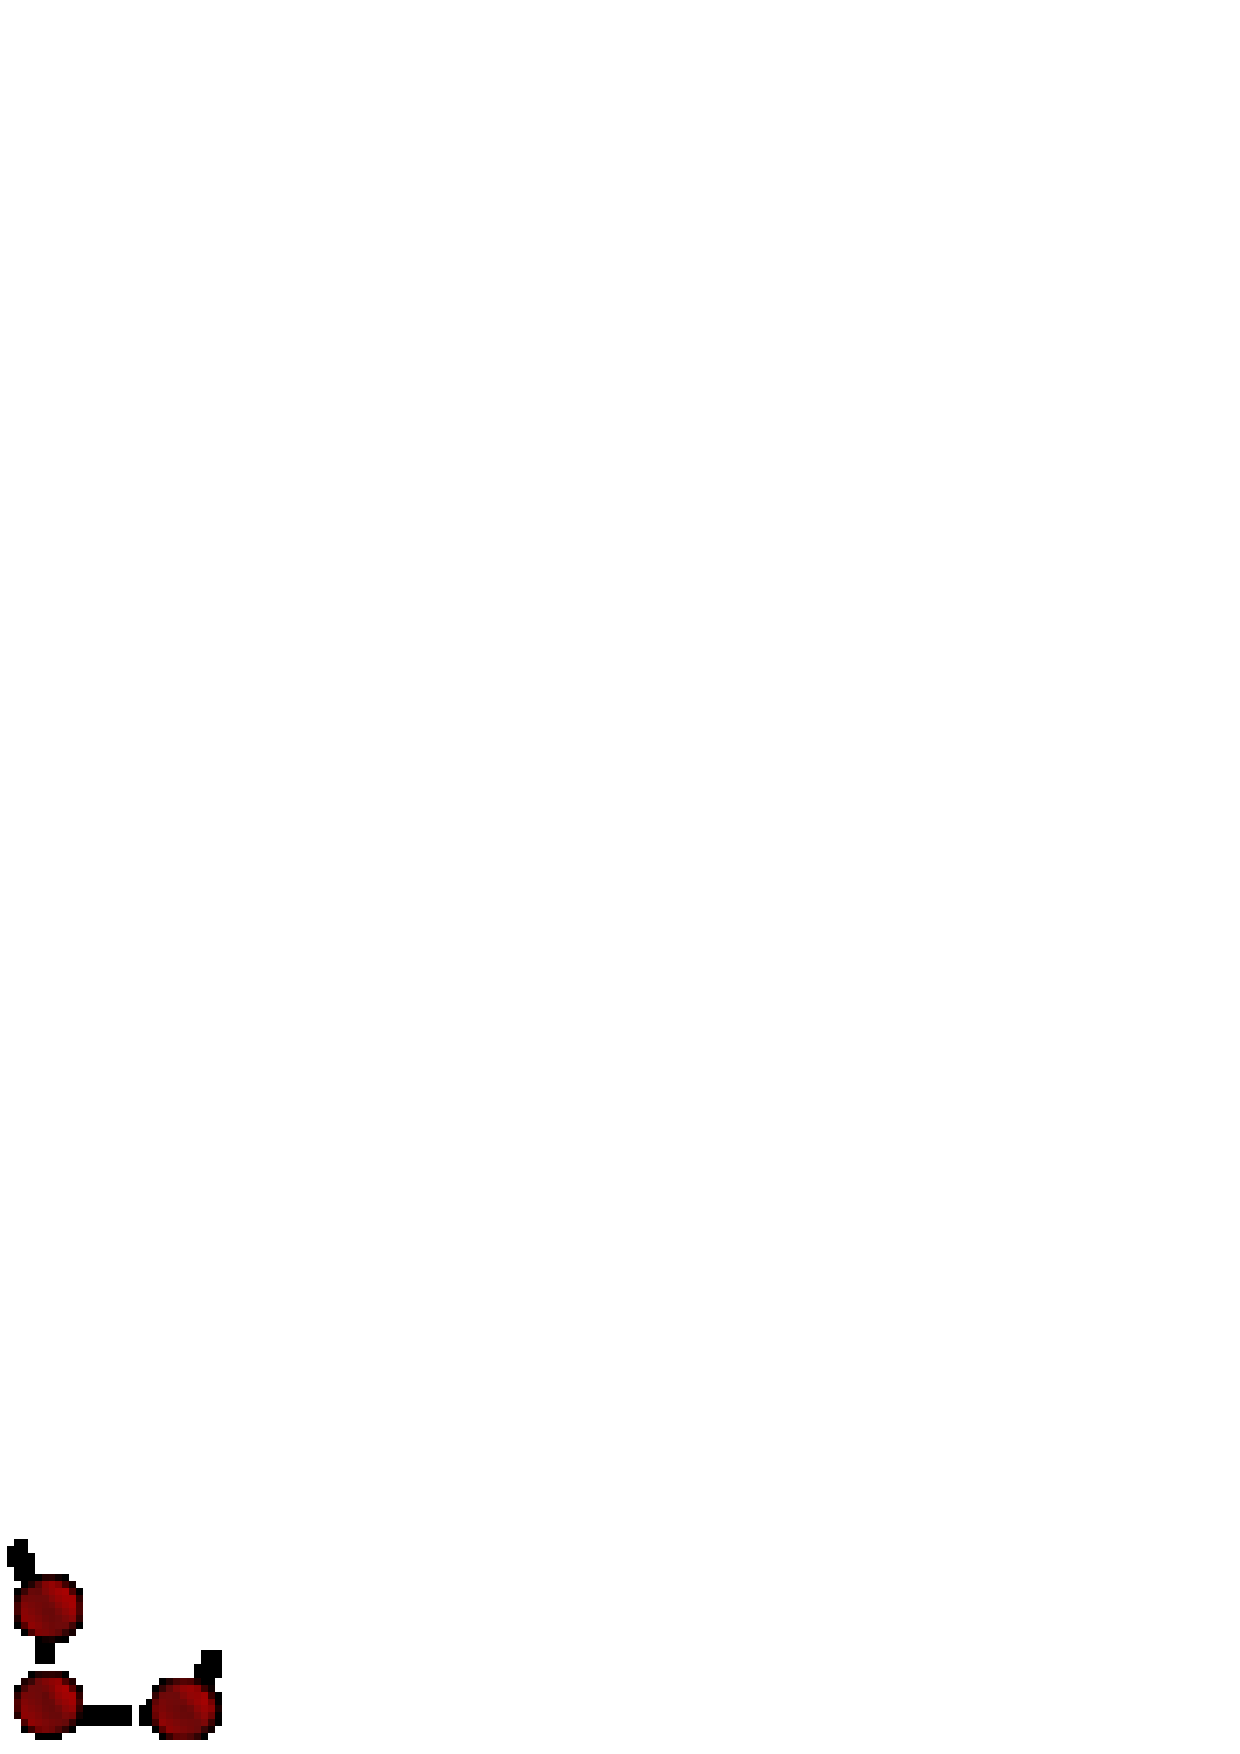
\includegraphics[width=0.7cm]{grass_new_line} & Nouvelle Ligne & Numérise une nouvelle ligne (terminez la numérisation en sélectionnant un nouvel outil) \\
\hline 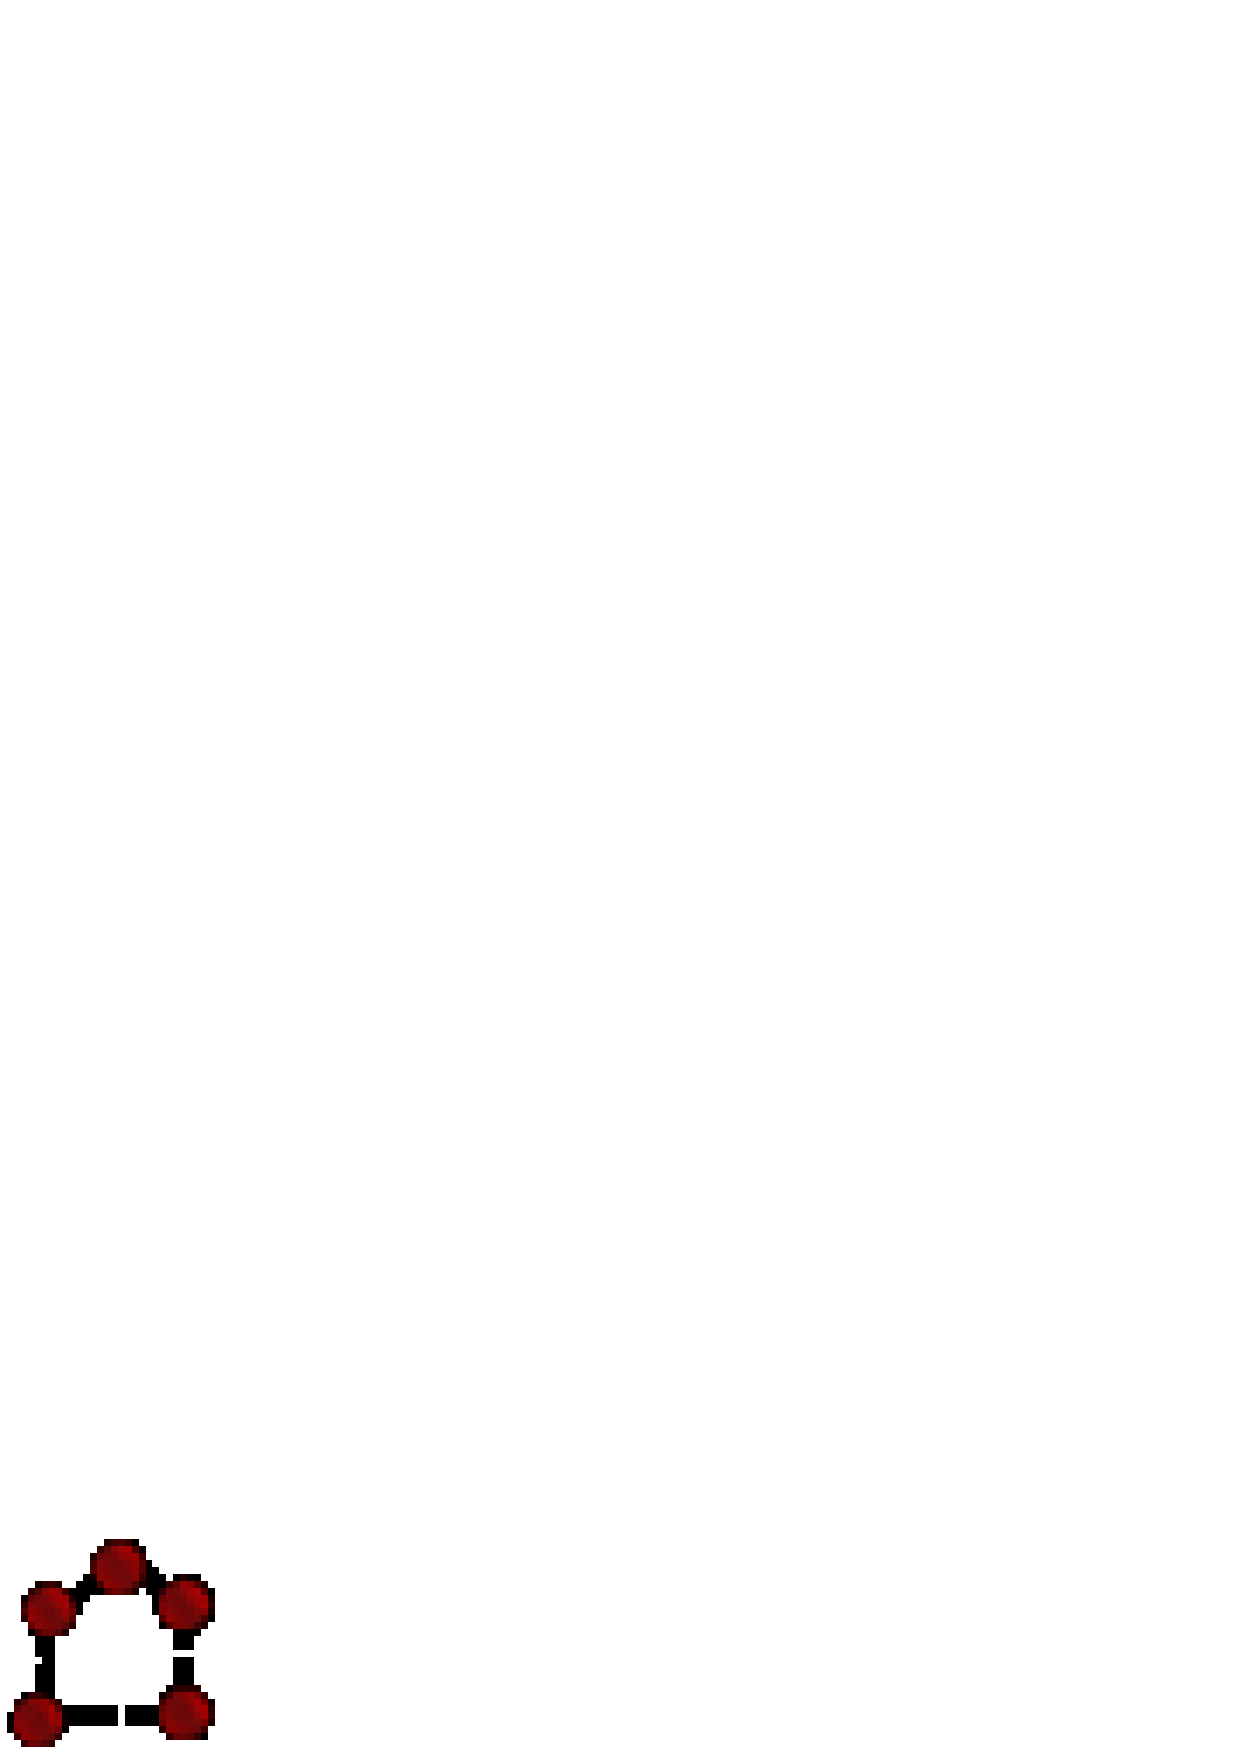
\includegraphics[width=0.7cm]{grass_new_boundary} & Nouveau Contour & Numérise un nouveau contour (terminer la numérisation en sélectionnant un nouvel outil)\\
\hline 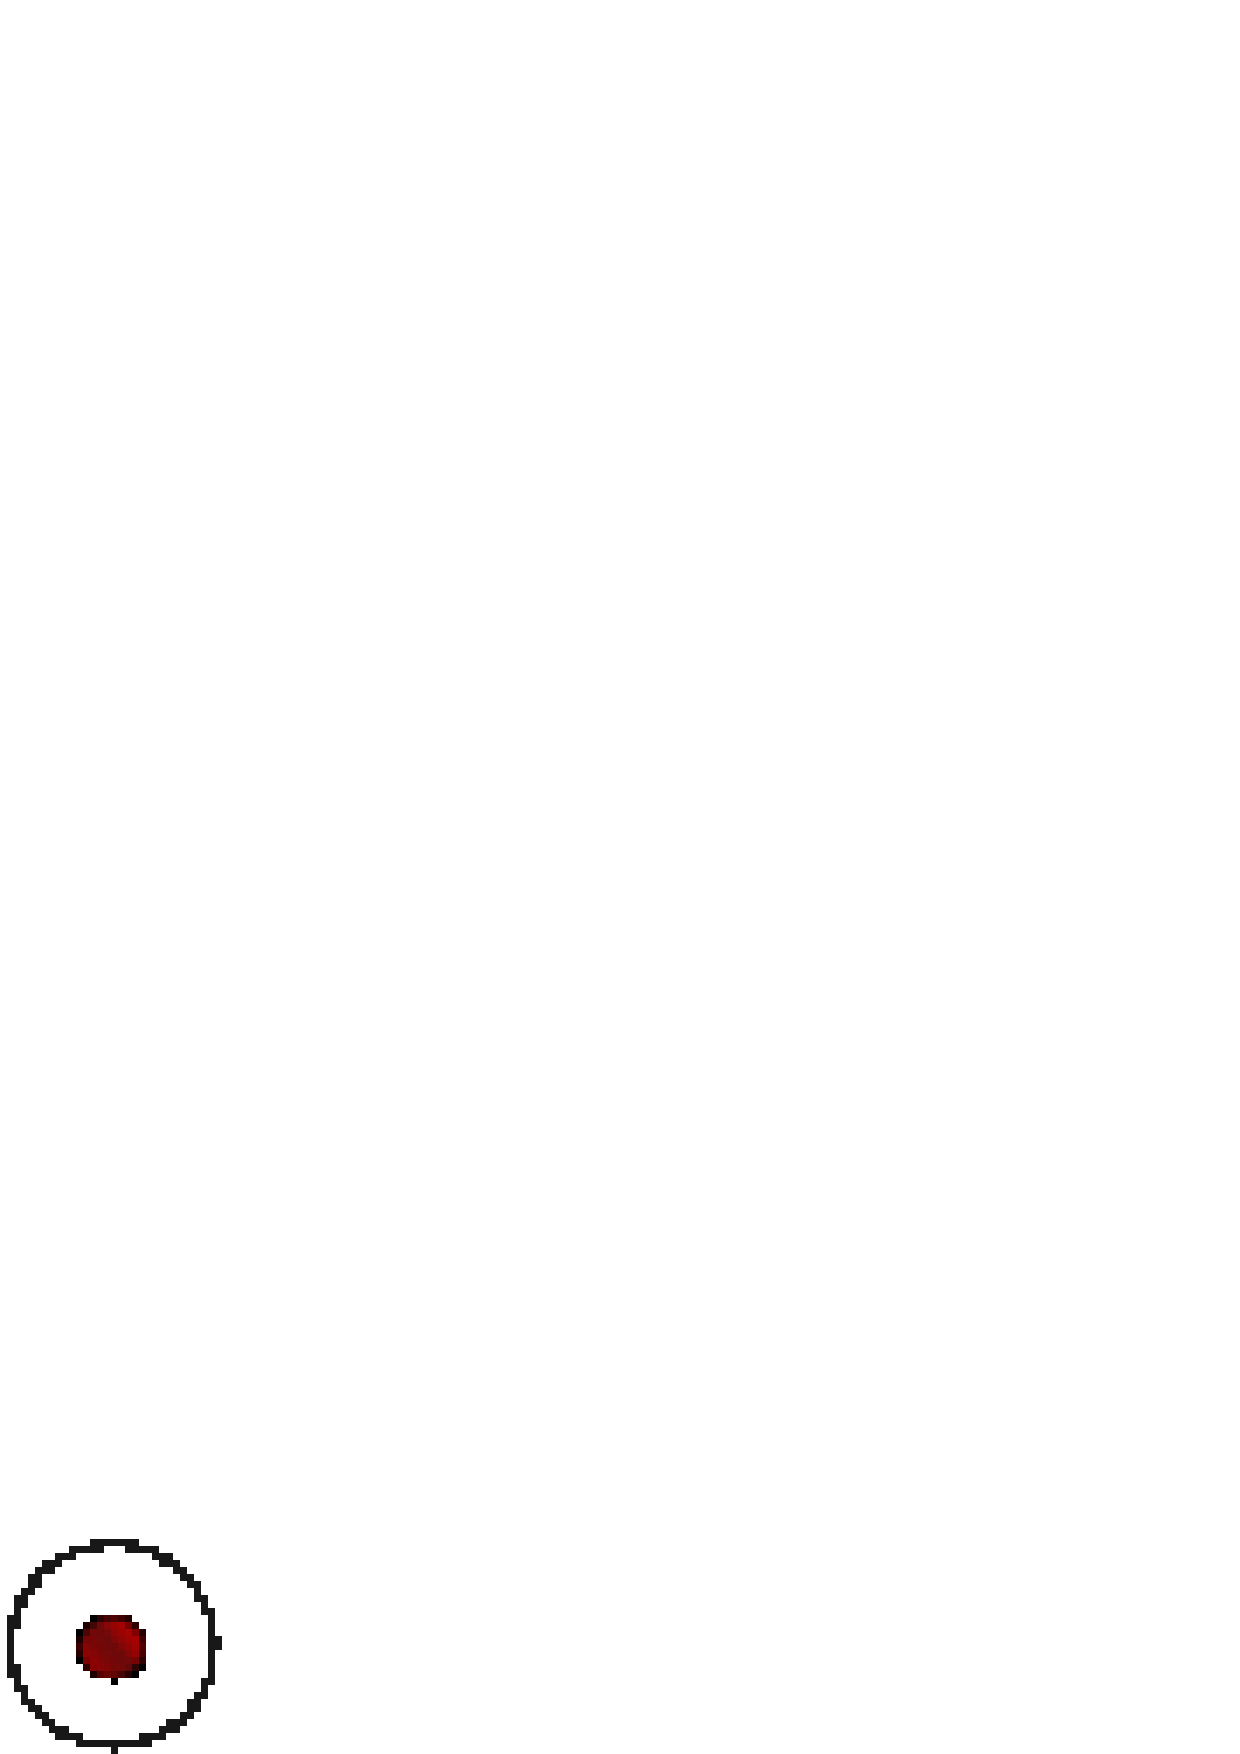
\includegraphics[width=0.7cm]{grass_new_centroid} & Nouveau Centroïde & Numérise un nouveau centroïde (emplacement de l'étiquette d'un polygone existant)\\
\hline 
\includegraphics[width=0.7cm]{grass_move_vertex} & Déplacer le sommet & Déplace un sommet d'une ligne ou d'un polygone existant et indique sa nouvelle position\\
\hline 
\includegraphics[width=0.7cm]{grass_add_vertex} & Ajouter un sommet & Ajoute un nouveau sommet à une ligne existante\\
\hline 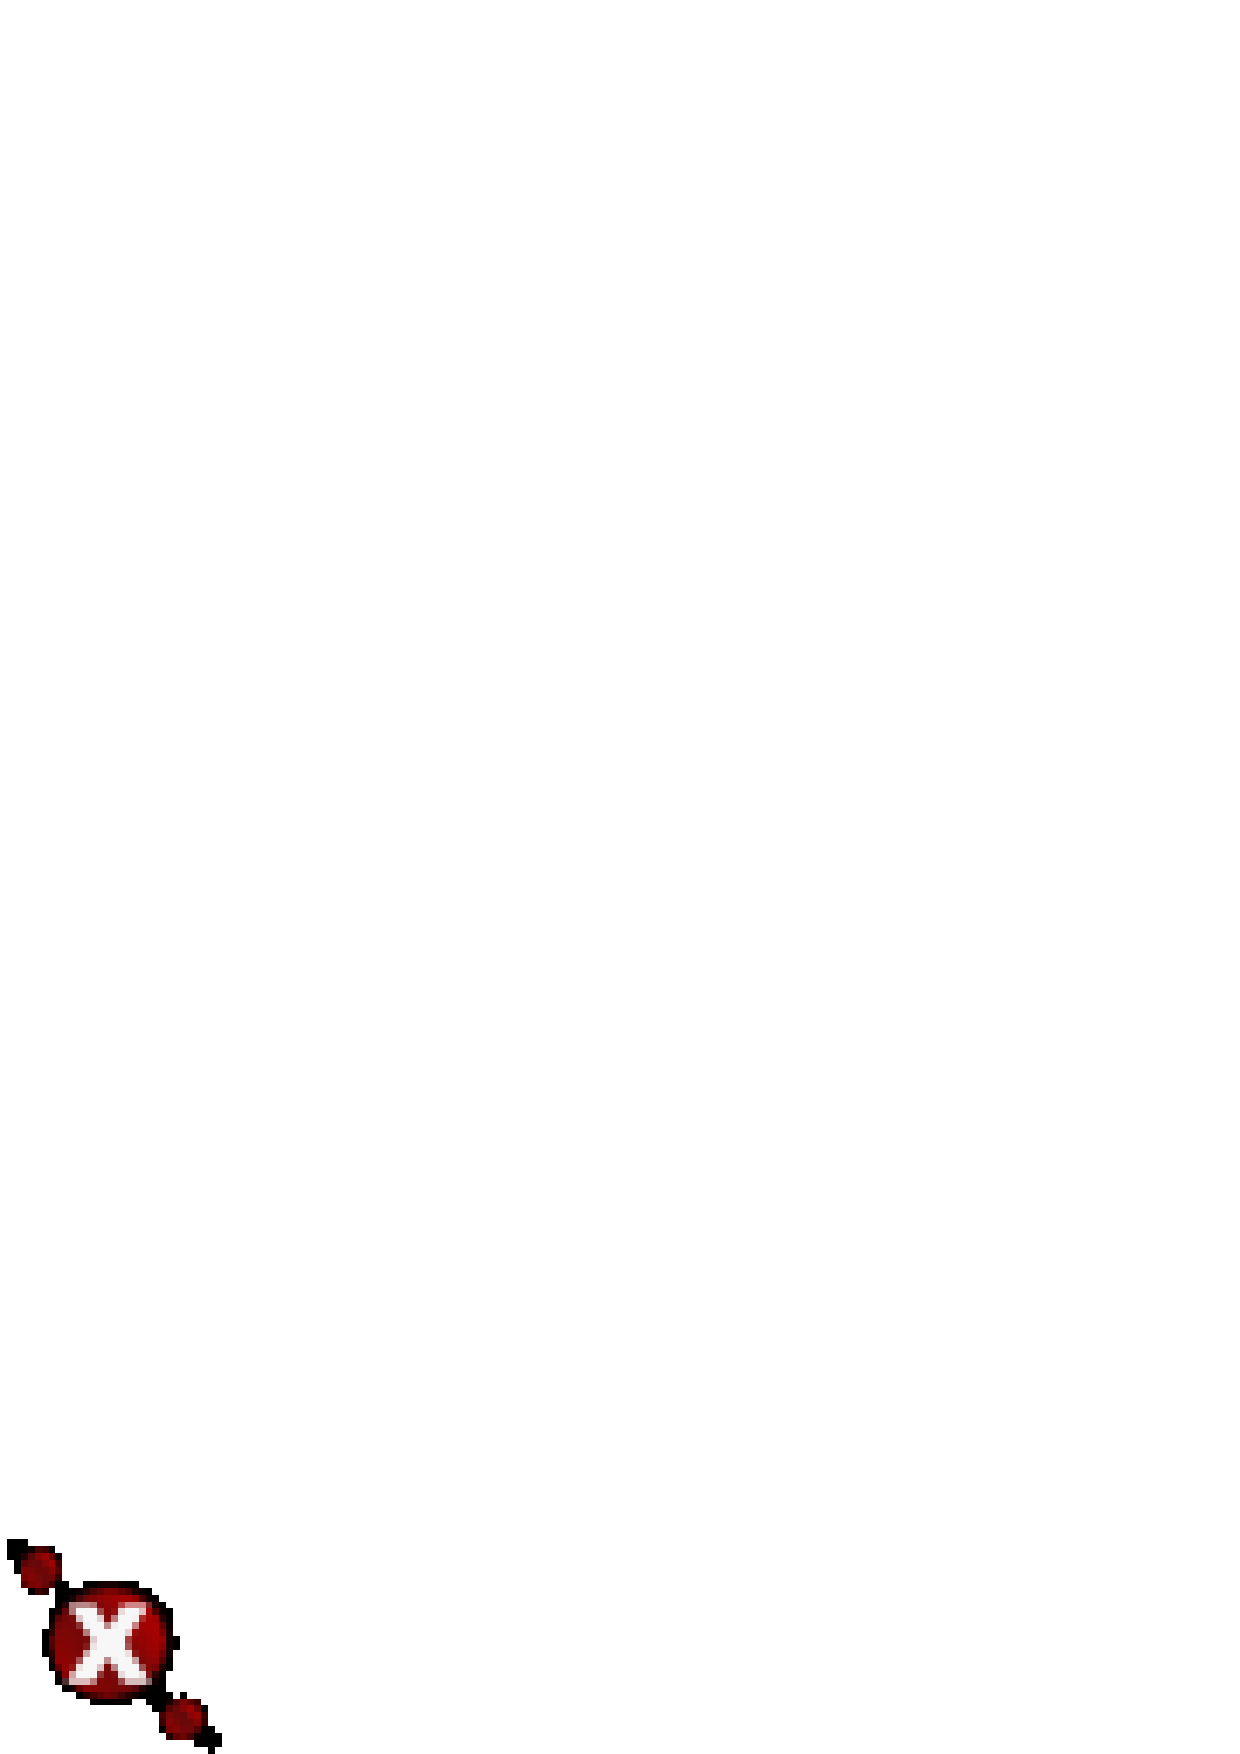
\includegraphics[width=0.7cm]{grass_delete_vertex} & Effacer un sommet & Efface un sommet d'une ligne existante (confirmez le sommet sélectionné avec un autre clic)\\
\hline 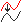
\includegraphics[width=0.7cm]{grass_move_line} & Déplace l'élément & Déplacez la limite, la ligne, le point ou le centroïde sélectionné puis cliquez sur la nouvelle position\\
\hline 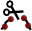
\includegraphics[width=0.7cm]{grass_split_line} & Coupe la ligne & Coupe une ligne existante en deux parties\\
\hline 
\includegraphics[width=0.7cm]{grass_delete_line} & Efface l'élément & Efface une limite, une ligne, un point ou un centroïde existant (confirmez l'élément sélectionné avec un autre clic)\\
\hline 
\includegraphics[width=0.7cm]{grass_edit_attributes} & Éditer les attributs & Édite les attributs de l'élément sélectionné (notez qu'un seul élément peut représenter plusieurs géométries, voir ci-dessus)\\
\hline 
\includegraphics[width=0.7cm]{grass_close_edit} & Fermer & Ferme la session et sauvegarde l'état actuel (reconstruit la topologie après)\\
\hline
\end{tabular}
\caption{\grass Digitizing Tools}\label{tab:grass_tools}
\end{table}}

%\minisec{Category Tab}\index{\grass!category settings}
\minisec{Onglet Categorie}\index{\grass!paramètres de catégorie}
%The \tab{Category} tab allows you to define the way in which the category values will be assigned to a new geometry element.
L'onglet \tab{Categorie} vous permet de définir la manière dont les valeurs du champ category sont assignées au nouvel élément géométrique.

\begin{figure}[ht]
 \begin{center}
  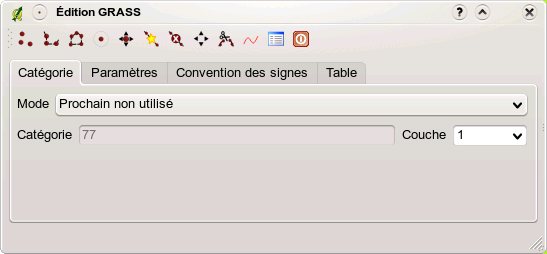
\includegraphics[clip=true,width=10cm]{grass_digitizing_category}
  \caption{Onglet Catégorie d'Édition \grass \nixcaption}\label{fig:grass_digitizing_category}
 \end{center}
\end{figure}

\begin{description}
%\item \textbf{Mode}: what category value shall be applied to new geometry elements.
\item[Mode :]quelle catégorie sera appliquée au nouvel élément.
\begin{itemize}[label=--]
%\item Next not used - apply next not yet used category value to geometry element.
\item Prochain non utilisé - applique la valeur suivante non utilisée du champ category à l'élément géométrique.
%\item Manual entry - manually define the category value for the geometry element in the 'Category'-entry field.
\item Saisie manuelle - saisir manuellement la valeur du champ category pour l'élément géométrique.
%\item No category - Do not apply a category value to the geometry element. This is e.g. used for area boundaries, because the category values are connected via the centroid.
\item Pas de catégorie - ne pas remplir le champ category. C'est par exemple utilisé pour les surfaces, car les valeurs de catégorie sont stockées via le centroïde
\end{itemize}
%\item \textbf{Category} - A number (ID) is attached to each digitized geometry element. It is used to connect each geometry element with its attributes.
\item[Categorie :]un identifiant (ID) est attaché à chaque objet numérisé. Il est utilisé pour connecter les objets géométriques avec ces attributs.
%\item \textbf{Field (layer)} - Each geometry element can be connected with several attribute tables using different \grass geometry layers. Default layer number is 1. 
\item[Couche :]Chaque objet peut être connecté à différentes tables attributaires au travers des différentes sous-couches. Le numéro de sous-couche par défaut est 1.
\end{description}

%\begin{Tip}\caption{\textsc{Creating an additional \grass 'layer' with \qg}}
\begin{Tip}\caption{\textsc{Création d'une sous-couche supplémentaire avec \qg}}
% \qgistip{If you would like to add more layers to your dataset, just add a new
% number in the 'Field (layer)' entry box and press return. In the Table tab
% you can create your new table connected to your new layer.
% }
Si vous souhaitez avoir plusieurs sous-couches dans votre couche vecteur, ajouter simplement un nouveau chiffre dans la zone de saisie 'Couche' et appuyez sur entrée. Dans l'onglet Table, vous pouvez créer de nouvelles tables attributaires connectées à votre nouvelle sous-couche.
\end{Tip}

%\minisec{Settings Tab}\label{label_settingtab}\index{\grass!snapping tolerance}
\minisec{Onglet Paramètres}\label{label_settingtab}\index{\grass!tolérance d'accrochage}

% The \tab{Settings} tab allows you to set the snapping in screen pixels. The
% threshold defines at what distance new points or line ends are snapped to
% existing nodes. This helps to prevent gaps or dangles between boundaries. The
% default is set to 10 pixels.

L'onglet \tab{Paramètres} vous permet de définir la tolérance d'accrochage en pixels-écrans. Le seuil définit à partir de quelle distance les nouveaux points ou les nouvelles lignes sont accrochées automatiquement à des noeuds existants. Cela aide à éviter de créer des trous ou des superpositions entre les contours. La valeur par défaut est fixée à 10 pixels.

\begin{figure}[ht]
 \begin{center}
 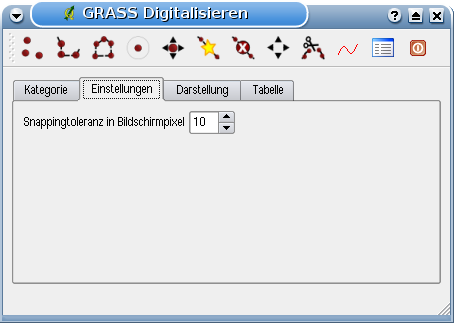
\includegraphics[clip=true,width=8cm]{grass_digitizing_settings}
 \caption{\grass Digitizing Settings Tab \nixcaption}\label{fig:grass_digitizing_settings}
 \end{center}
\end{figure}

%\minisec{Symbology Tab}\index{\grass!symbology settings}
\minisec{Onglet Convention des signes}\index{\grass!convention des signes}

% The \tab{Symbology} tab allows you to view and set symbology and color settings for various geometry types and their topological status (e.g. closed
% / opened boundary).
L'onglet \tab{Convention des signes} vous permet d'afficher et modifier la symbologie, la couleur des différentes formes géométriques ainsi que leur statut topologique (par exemple : contour ouvert / fermé)

\begin{figure}[ht]
 \begin{center}
 %\caption{\grass Digitizing Symbolog Tab \nixcaption}\label{fig:grass_digitizing_symbology}
 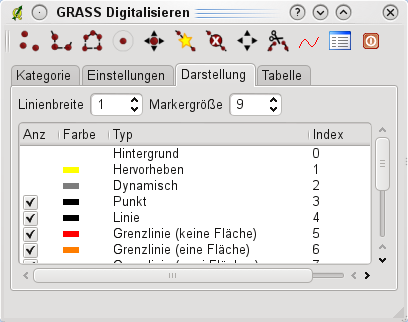
\includegraphics[clip=true,width=8cm]{grass_digitizing_symbology}
  \caption{Onglet Paramètres d'Édition \grass \nixcaption}\label{fig:grass_digitizing_settings}
 \end{center}
\end{figure}

%\minisec{Table Tab} \index{\grass!table editing}
\minisec{Onglet Table} \index{\grass!Éditer une table}
% The \tab{Table} tab provides information about the database table for
% a given 'layer'. Here you can add new columns to an existing attribute table,
% or create a new database table for a new \grass vector layer (see Section 
% \ref{sec:creating_new_grass_vectors}).
L'onglet \tab{Table} donne des informations sur la table attributaire d'une sous-couche donnée. C'est ici que vous pouvez ajouter des colonnes à une table attributaire existante ou créer une nouvelle table attributaire pour une nouvelle couche vectorielle \grass (voir Section \ref{sec:creating_new_grass_vectors}).

\begin{figure}[ht]
 \begin{center}
 %\caption{\grass Digitizing Table Tab \nixcaption}\label{fig:grass_digitizing_table}
 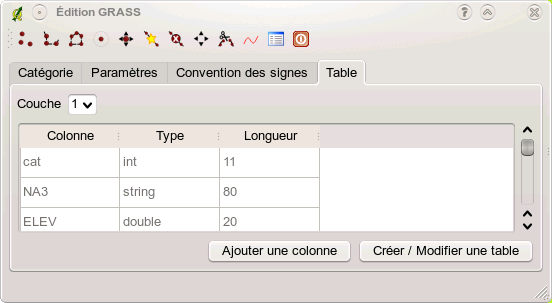
\includegraphics[clip=true,width=10cm]{grass_digitizing_table}
  \caption{Onglet Table du mode Édition \grass \nixcaption}\label{fig:grass_digitizing_table}
 \end{center}
\end{figure}

%\begin{Tip}\caption{\textsc{\grass Edit Permissions}}\index{\grass!edit permissions}
\begin{Tip}\caption{\textsc{Éditer les permissions \grass}}\index{\grass!éditer les permissions}
% \qgistip{You must be the owner of the \grass \filename{MAPSET} you want to 
% edit. It is impossible to edit data layers in a \filename{MAPSET} that is not 
% yours, even if you have write permissions.
% }
Vous devez être propriétaire du \filename{Jeu de données} que vous voulez éditer. Il est impossible de modifier des informations d'un \filename{Jeu de données} qui n'est pas à vous, même si vous avez des droits en écriture.
\end{Tip} 

%\section{The \grass region tool}\label{sec:grass_region}\index{\grass!region}
\section{L'outil région \grass}\label{sec:grass_region}\index{\grass!région}

%The region definition (setting a spatial working window) in \grass is important 
%for working with raster layers. Vector analysis is by default not limited
%to any defined region definitions. But all newly-created rasters will have the
%spatial extension and resolution of the currently defined \grass region,
%regardless of their original extension and resolution. The current \grass
%region is stored in the \filename{\$LOCATION/\$MAPSET/WIND} file, and it 
%defines north, south, east and west bounds, number of columns and rows, 
%horizontal and vertical spatial resolution.

La définition d'une région (définir une emprise spatiale de travail) dans \grass est très importante pour travailler avec des couches rasters. Le travail d'analyse vecteur n'est, par défaut, pas limitée à une région définie. Mais, tous les rasters nouvellement créés auront l'extension spatiale et la résolution de la région \grass en cours d'utilisation, indépendamment de leur extension et résolution d'origine. La région courante \grass est stockée dans le fichier \filename{\$LOCATION/\$MAPSET/WIND}, et celui-ci définit les limites Nord, Sud, Est et Ouest, le nombre de lignes et de colonnes ainsi que la résolution spatiale horizontale et verticale.

% It is possible to switch on/off the visualization of the \grass region in the
% \qg canvas using the \toolbtntwo{grass_region}{Display current \grass region}
% button. \index{\grass!region!display}.
Il est possible de d'afficher ou de masquer l'affichage de la région \grass dans \qg à l'aide du bouton\toolbtntwo{grass_region}{Afficher la région courante \grass}. \index{\grass!région!afficher}.

% With the \toolbtntwo{grass_region_edit}{Edit current \grass region} icon you 
% can open a dialog to change the current region and the symbology of the \grass 
% region rectangle in the \qg canvas. Type in the new region bounds and 
% resolution and click \button{OK}. It also allows to select a new region 
% interactively with your mouse on the \qg canvas. Therefore click with the 
% left mouse button in the \qg canvas, open a rectangle, close it using the 
% left mouse button again and click \button{OK}.\index{\grass!region!editing}
% The \grass module \filename{g.region} provide a lot more parameters to define 
% an appropriate region extend and resolution for your raster analysis. You can 
% use these parameters with the \grass Toolbox, described in Section 
% \ref{subsec:grass_toolbox}.

A l'aide du bouton \toolbtntwo{grass_region_edit}{Éditer la région courante \grass} vous avez accès à une boîte dialogue qui vous permet de modifier la région courante ainsi que sa symbologie. Entrez les nouvelles limites et résolution et cliquez sur \button{OK}. Cette boîte de dialogue vous permet aussi de définir une nouvelle région interactivement à l'aide de la souris. Pour définir ce rectangle d'emprise, cliquez avec le bouton gauche de la souris et définissez un rectangle que vous terminerez en cliquant de nouveau sur le bouton gauche de la souris et fermez la boîte de dialogue en cliquant sur \button{OK}.\index{\grass!région!éditer} Le module \grass \filename{g.region} propose un grand nombre de paramètres pour définir de façon appropriée les limites et la résolution d'une région pour faire de l'analyse raster. Vous pouvez vous servir de ces paramètres dans la boîte à outils \grass décrite dans la section \ref{subsec:grass_toolbox}.

%\section{The \grass toolbox}\label{subsec:grass_toolbox}\index{\grass!toolbox}
\section{La boîte à outils \grass}\label{subsec:grass_toolbox}\index{\grass!boîte à outils}

% The \toolbtntwo{grass_tools}{Open \grass Tools} box provides \grass module 
% functionalities to work with data inside a selected \grass \filename{LOCATION} 
% and \filename{MAPSET}. To use the \grass toolbox you need to open a 
% \filename{LOCATION} and \filename{MAPSET} where you have write-permission 
% (usually granted, if you created the \filename{MAPSET}). This is necessary, 
% because new raster or vector layers created during analysis need to be written 
% to the currently selected \filename{LOCATION} and \filename{MAPSET}.

La boîte de dialogue \toolbtntwo{grass_tools}{Ouvrir les outils \grass} donne accès aux fonctionnalités \grass qui permettent de travailler dans un \filename{SECTEUR} et sur un \filename{Jeu de Données}. Pour utiliser les outils \grass, vous devez ouvrir un \filename{SECTEUR} et un \filename{Jeu de Données} sur lequel vous avez des droits d'écriture (que vous avez normalement si vous avez créé le \filename{Jeu de Données}). Cela est nécessaire car les rasters et les vecteurs nouvellement créés lors des analyses doivent être écrits dans le \filename{SECTEUR} et \filename{Jeu de Données} courant

%\subsection{Working with \grass modules}\label{grass_modules}\index{\grass!toolbox}
\subsection{Travailler avec les modules \grass}\label{grass_modules}\index{\grass!boîte à outils}
\begin{figure}[ht]
\centering
% \caption{\grass Toolbox and searchable Modules List \nixcaption}\label{fig:grass_modules}
   % \subfigure[Modules Tree] {\label{subfig:grass_module_tree}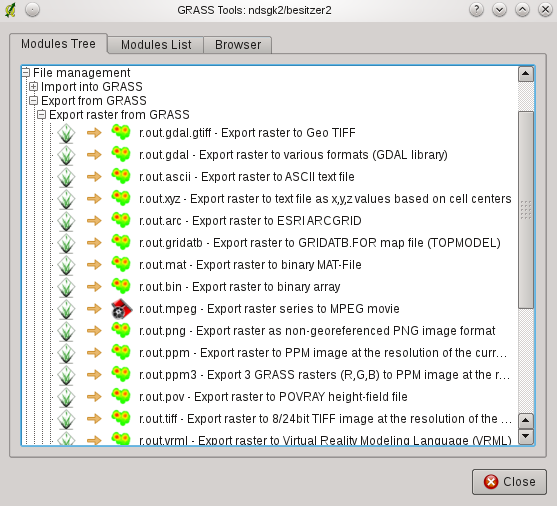
\includegraphics[clip=true, width=0.4\textwidth]{grass_toolbox_moduletree}}\goodgap
   % \subfigure[Searchable Modules List] {\label{subfig:grass_module_list}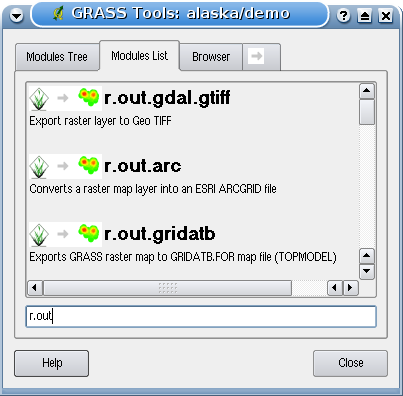
\includegraphics[clip=true, width=0.4\textwidth]{grass_toolbox_modulelist}}
   \subfloat[Arborescence des modules] {\label{subfig:grass_module_tree}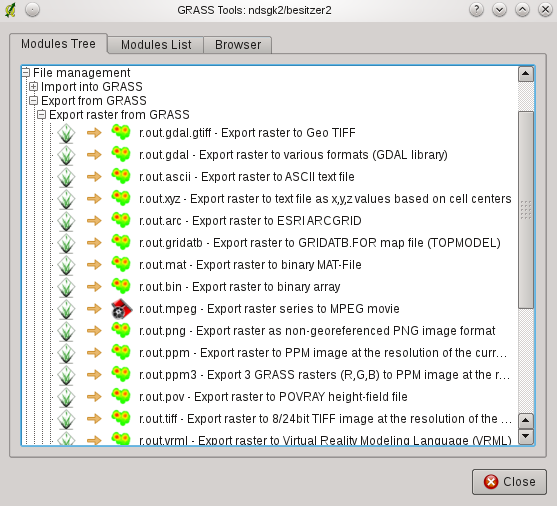
\includegraphics[clip=true, width=0.4\textwidth]{grass_toolbox_moduletree}}
   \hspace{0.5cm}
   \subfloat[Liste des modules avec possibilité de recherche] {\label{subfig:grass_module_list}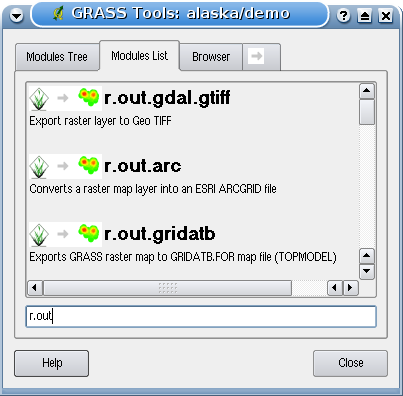
\includegraphics[clip=true, width=0.4\textwidth]{grass_toolbox_modulelist}}   
\caption{Outils \grass et Liste des Modules \nixcaption}\label{fig:grass_modules}
\end{figure}

% The \grass Shell inside the \grass Toolbox provides access to almost all (more 
% than 300) \grass modules in command line modus. To offer a more user
% friendly working environment, about 200 of the available \grass modules and 
% functionalities are also provided by graphical dialogs. These dialogs are 
% grouped in categories, but are searchable as well. You find a complete 
% list of \grass modules available in \qg version \CURRENT
% in appendix \ref{appdx_grass_toolbox_modules}. It is also possible to 
% customize the \grass Toolbox content. It is described in Section 
% \ref{sec:toolbox-customizing}.
L'invite de commande de la boîte à outils \grass vous donne accès à pratiquement tous les modules \grass (près de 300) en ligne de commande. Afin d'offrir un environnement de travail plus agréable, environ 200 d'entre eux sont fournis avec une boîte de dialogue. Ces boîtes de dialogue sont groupées par catégories mais sont aussi accessibles par une recherche libre. Vous trouverez une liste complète des modules \grass disponibles dans \qg \CURRENT dans l'annexe \ref{appdx_grass_toolbox_modules}. Il est aussi possible de personnaliser le contenu de la boîte à outils \grass. Ceci est décrit dans la section \ref{sec:toolbox-customizing}.

% As shown in Figure \ref{fig:grass_modules}, you can look for the appropriate 
% \grass module using the thematically grouped \tab{Modules Tree} or the 
% searchable \tab{Modules List} tab. 
Comme indiqué sur la figure \ref{fig:grass_modules}, vous pouvez chercher le module \grass approprié en utilisant l'onglet \tab{Arborescence des modules} ou en utilisant l'onglet \tab{Liste des Modules} pour faire une recherche.
% Clicking on a grapical module icon a new tab will be added to the toolbox 
% dialog providing three new sub-tabs \tab{Options}, \tab{Output} and 
% \tab{Manual}. In Figure \ref{fig:grass_module_dialog} you see an example 
% for the \grass module \filename{v.buffer}.
Lorsque vous cliquez sur un module, un nouvel onglet apparaît proposant trois sous-onglets \tab{Options}, \tab{Rendu} et \tab{Manuel}. Sur la figure \ref{fig:grass_module_dialog}, vous voyez un exemple pour le module \grass \filename{v.buffer}.

\begin{figure}[ht]
\centering
% \caption{\grass Toolbox Module Dialogs \nixcaption}\label{fig:grass_module_dialog}
   % \subfigure[Module Options] {\label{subfig:grass_module_option}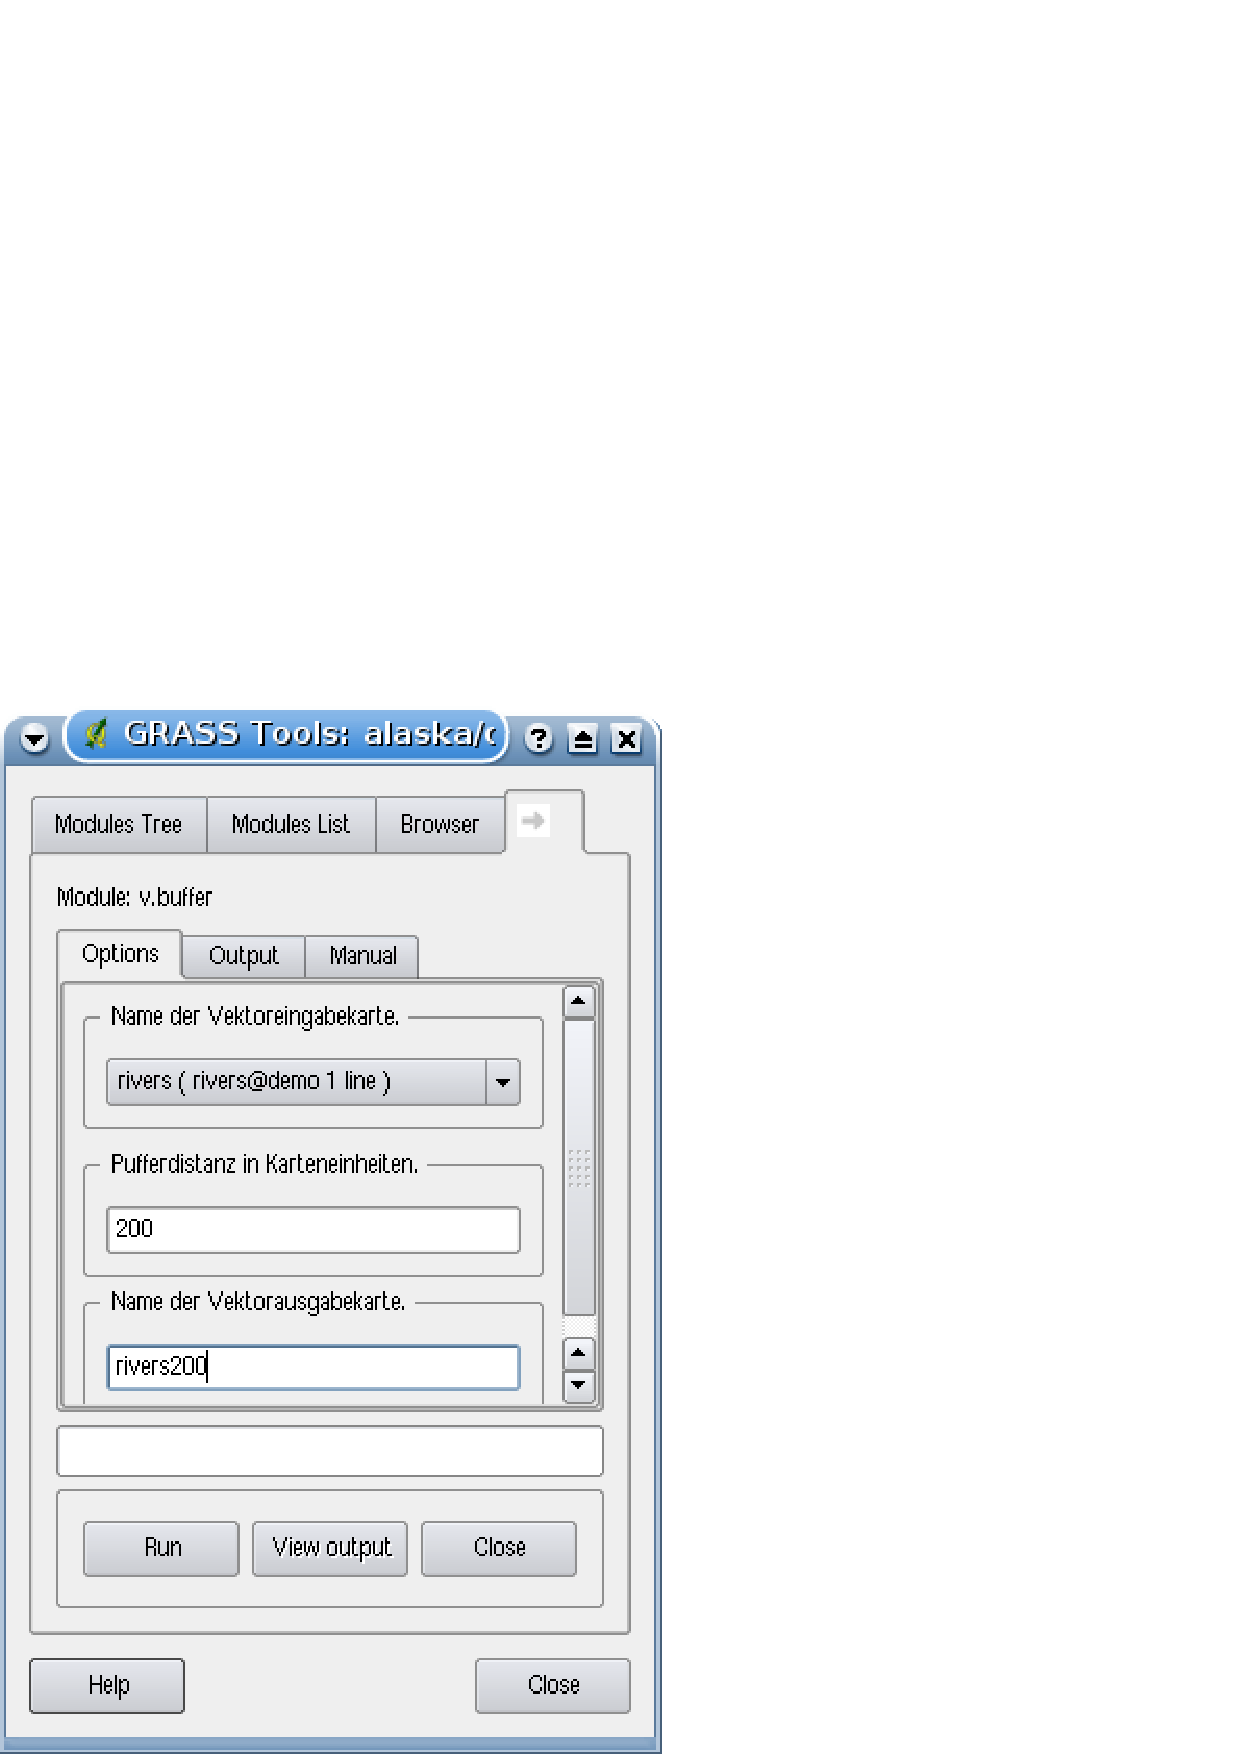
\includegraphics[clip=true, width=0.3\textwidth]{grass_module_option}}\goodgap
   % \subfigure[Modules Output] {\label{subfig:grass_module_output}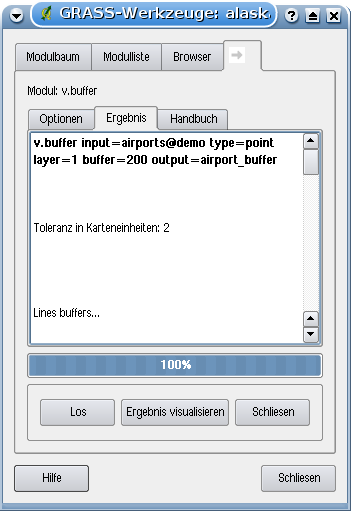
\includegraphics[clip=true, width=0.3\textwidth]{grass_module_output}}\goodgap
   % \subfigure[Module Manual] {\label{subfig:grass_module_manual}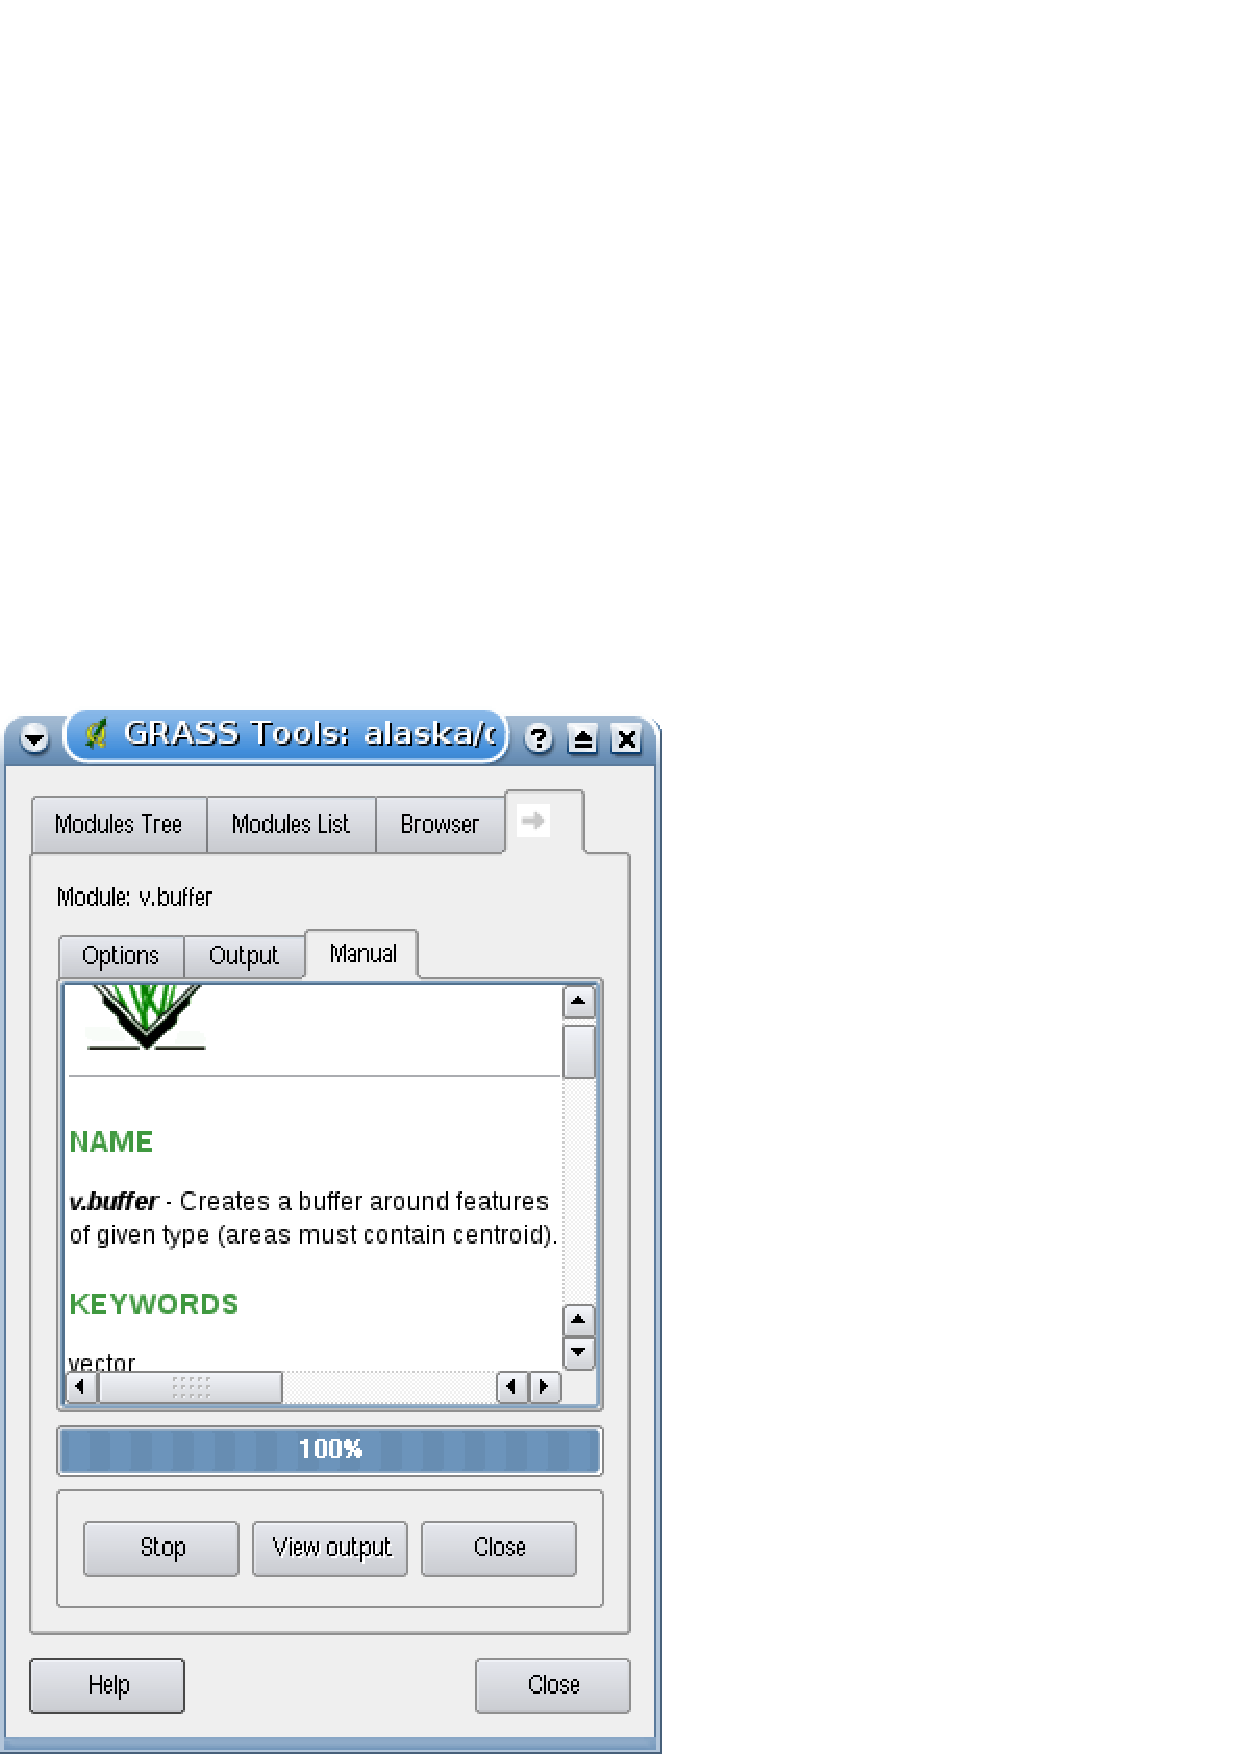
\includegraphics[clip=true, width=0.3\textwidth]{grass_module_manual}}
   \subfloat[Options du module] {\label{subfig:grass_module_option}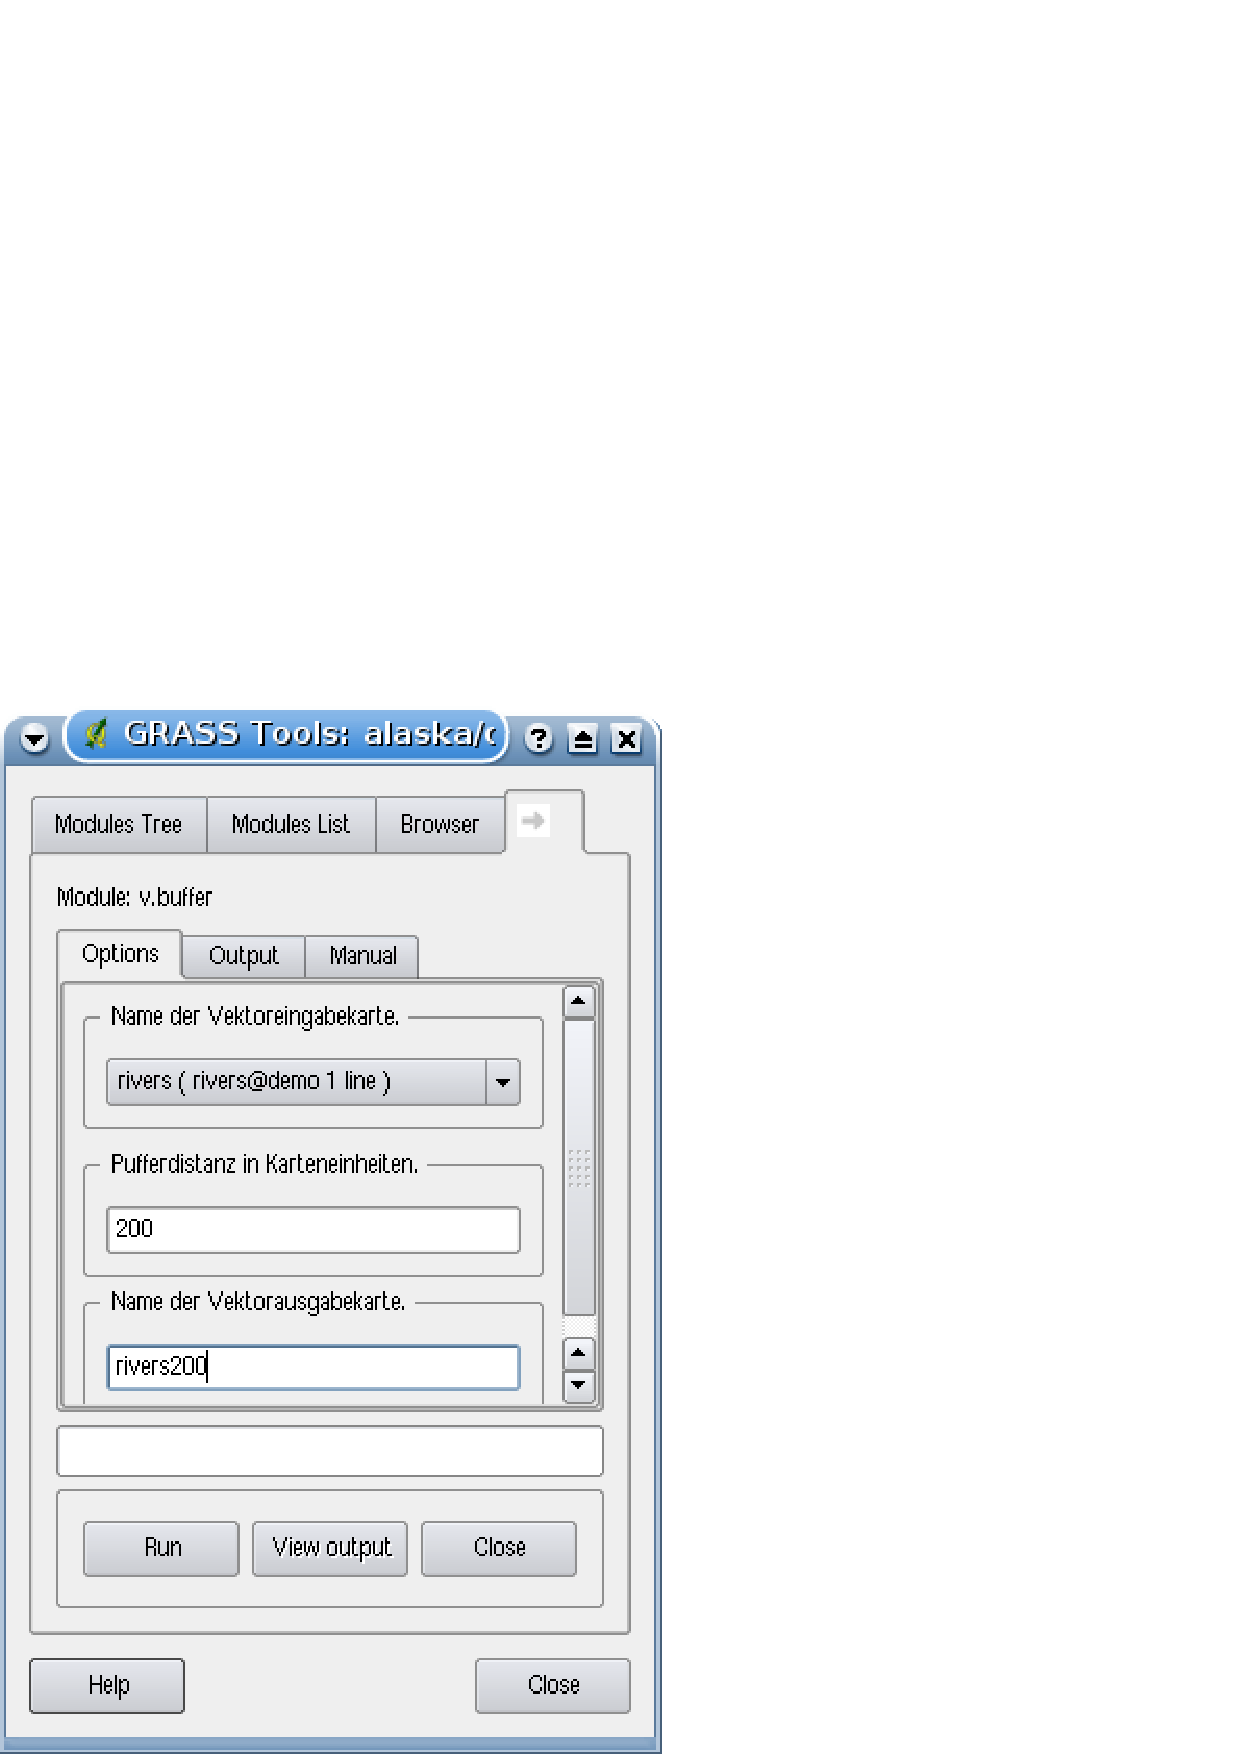
\includegraphics[clip=true, width=0.3\textwidth]{grass_module_option}}
   \hspace{0.2cm}
   \subfloat[Rendu du module] {\label{subfig:grass_module_output}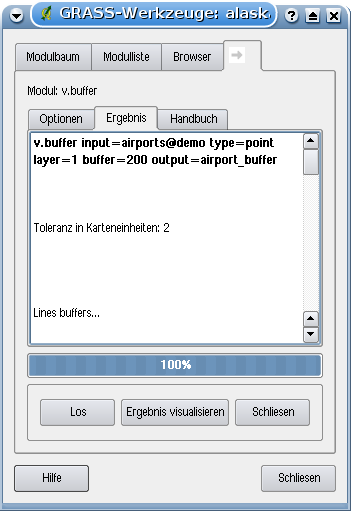
\includegraphics[clip=true, width=0.3\textwidth]{grass_module_output}}
    \hspace{0.2cm}
   \subfloat[Aide sur le module] {\label{subfig:grass_module_manual}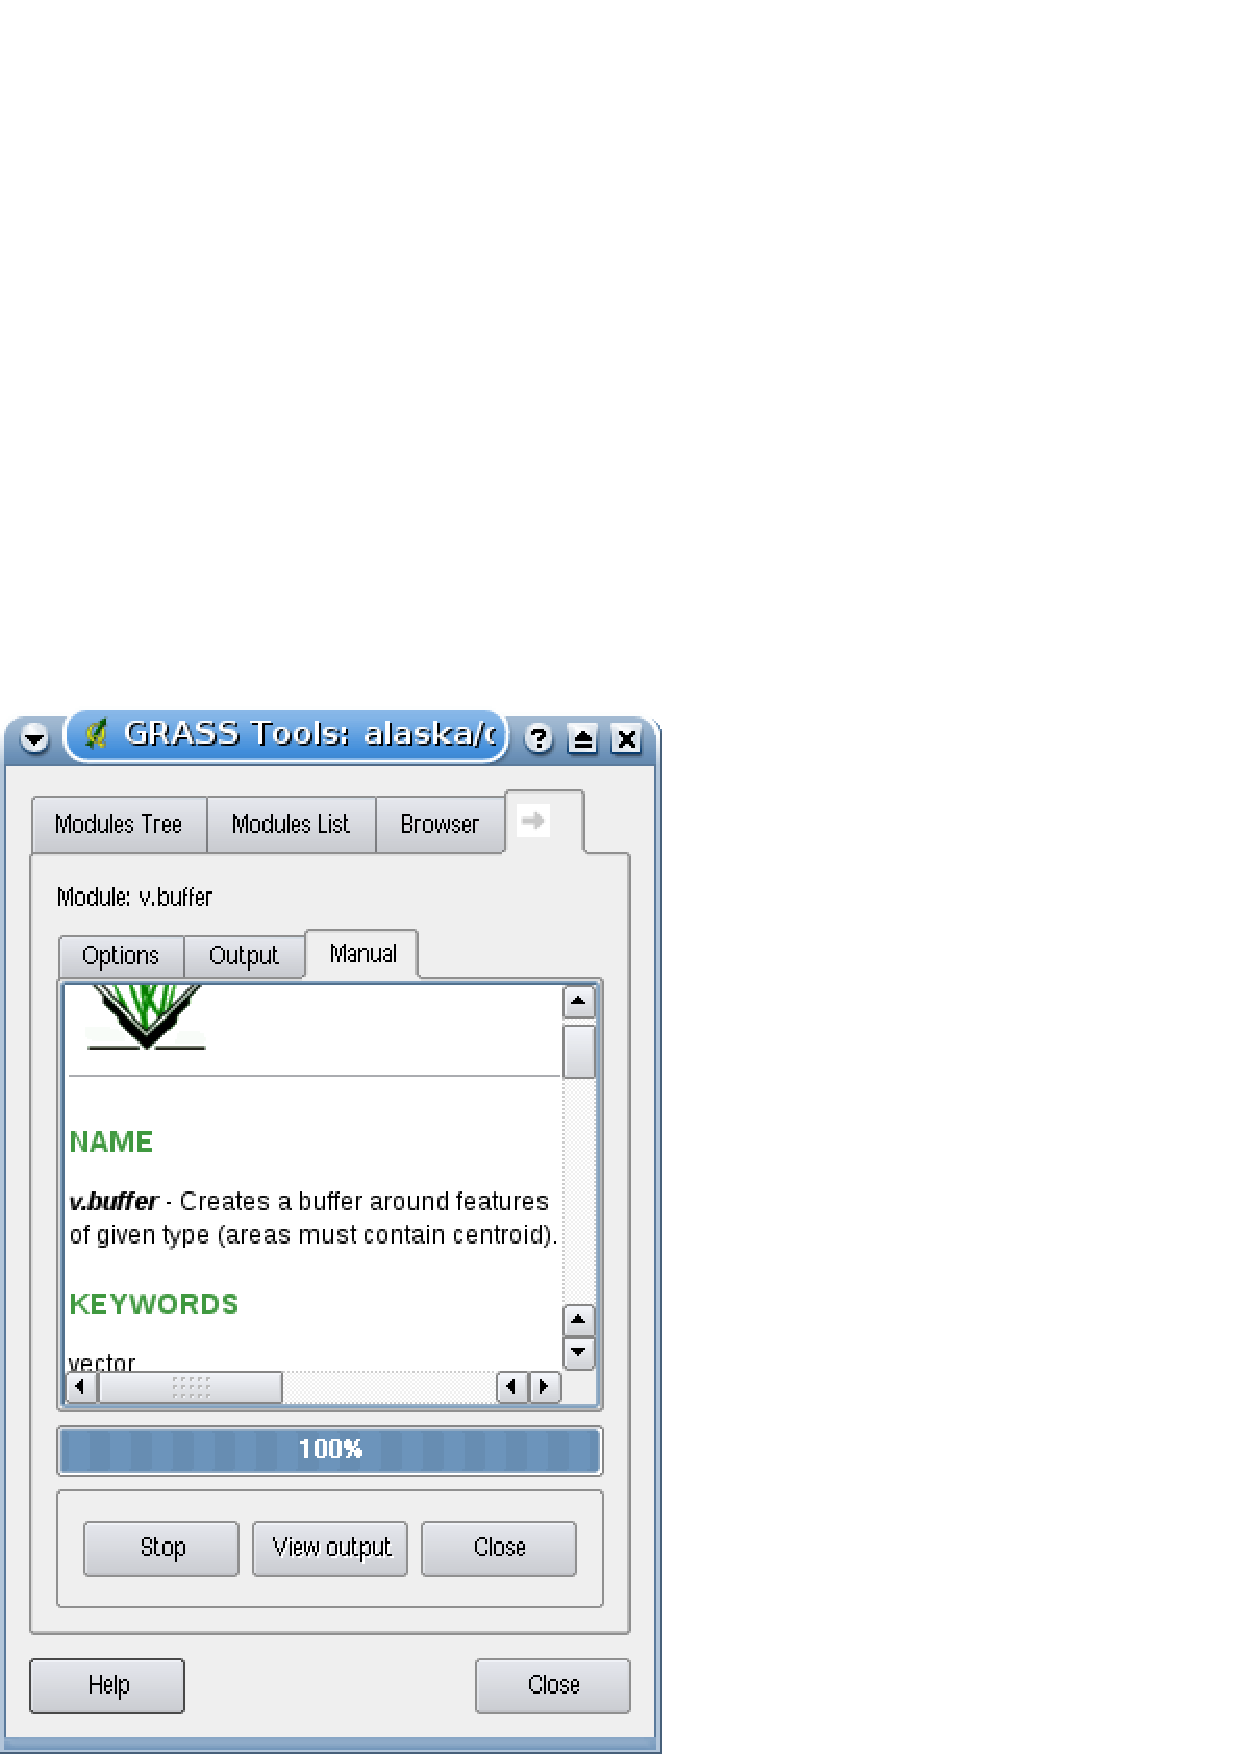
\includegraphics[clip=true, width=0.3\textwidth]{grass_module_manual}}
 \caption{Boîte de dialogue d'un module issue des outils \grass \nixcaption}\label{fig:grass_module_dialog}  
\end{figure}

\minisec{Options}

% The \tab{Options} tab provides a simplified module dialog where you can 
% usually select a raster or vector layer visualized in the \qg canvas and 
% enter further module specific parameters to run the module. The provided 
% module parameters are often not complete to keep the dialog clear. If you want 
% to use further module parameters and flags, you need to start the \grass Shell 
% and run the module in the command line.
L'onglet \tab{Options} propose une interface simplifiée où vous pouvez sélectionner un raster ou un vecteur en cours de visualisation dans \qg et
saisir les paramètres spécifiques au module avant de le lancer. Tous les paramètres du module ne sont généralement pas fournis afin de simplifier
les boîtes de dialogue. Pour utiliser des paramètres que ne se trouvent pas dans la boîte de dialogue, vous devez utiliser l'invite de commande
et lancer les modules en lignes de commande.

%A new feature in QGIS \CURRENT is the support for a 
%\button{show advanced options >>} button below the simplified module dialog 
%in the \tab{Options} tab. At the moment it is only added to the module v.in.ascii 
%as an example use, but will probably be part of more / all modules in the 
%GRASS toolbox in future versions of QGIS. This allows to use the complete GRASS 
%module options without the need to switch to the GRASS Shell.  

Une nouvelle fonctionnalité de \qg \CURRENT est l'ajout d'un bouton \button{afficher les options avancées >>} en-dessous du dialogue simplifié du panneau \tab{Options}. Pour l'instant seul le module v.in.ascii a été adapté afin de servir d'exemple d'utilisation mais d'autres le seront dans les prochaines versions de \qg. La finalité est de pouvoir recourir à toutes les options de GRASS dans devant ouvrir la console de commande (le shell).

%\minisec{Output}
\minisec{Rendu}

%The \tab{Output} tab provides information about the output status of the module. When you click the \button{Lancer} button, the module switches to the 
%\tab{Output} tab and you see information about the analysis process. If all works well, you will finally see a \usertext{Successfully finished} message.
L'onglet \tab{Rendu} fournit des informations sur l'état de sortie du module. Quand vous cliquez sur le bouton \button{Lancer}, le module passe sur l'onglet \tab{Rendu} et vous voyez les informations sur le processus en cours. Si tout se passe bien, vous verrez finalement le message \usertext{Terminé avec succès}.
%\minisec{Manual}
\minisec{Manuel}

% The \tab{Manual} tab shows the HTML help page of the \grass module. You can 
% use it to check further module parameters and flags or to get a deeper 
% knowledge about the purpose of the module. At the end of each module 
% manual page you see further links to the \filename{Main Help index}, the 
% \filename{Thematic index} and the \filename{Full index}. These links provide 
% the same information as if you use the module \filename{g.manual} 

L'onglet \tab{Manuel} montre la page HTML d'aide du module. Vous pouvez vous en servir pour voir les autres paramètres du modules et pour avoir une
connaissance plus approfondie de l'objet du module. A la fin de chaque page d'aide d'un module, vous avez des liens vers \filename{Main Help index} (table principale des matières), \filename{Thematic index}(par thèmes) et \filename{Full index}(l'index complet). Ces liens vous donnent les mêmes informations que si vous utilisiez directement \filename{g.manual}.

%\begin{Tip}\caption{\textsc{Display results immediately}}\index{\grass!display results}
\begin{Tip}\caption{\textsc{Afficher les résultats immédiatement}}\index{\grass!afficher les résultats}
%\qgistip{If you want to display your calculation results immediately in your map canvas, you can use the 'View Output' button at the bottom of the module tab.
Si vous voulez voir immédiatement dans votre fenêtre carte le résultat des calculs du module, vous pouvez utiliser le bouton 'Vue' au bas de l'onglet du module.
\end{Tip} 

%\subsection{\grass module examples}\index{\grass!toolbox}
\subsection{Exemples de modules \grass }\index{\grass!boîte à outils}
%The following examples will demonstrate the power of some of the \grass modules. 
Les exemples suivants décriront les possibilités de certains modules \grass.

%\minisec{Creating contour lines}
\minisec{Création de courbes de niveau} 

%The first example creates a vector contour map from an elevation raster (DEM). Assuming you have the Alaska \filename{LOCATION} set up as explained
%in Section \ref{sec:import_loc_data}. 
Le premier exemple créé un couche vecteur de courbe de niveau à partir d'un modèle numérique de terrain (MNT). Nous considérerons que le jeu de données exemple \filename{SECTEUR} a été installé comme décrit au paragraphe \ref{sec:import_loc_data}.

\begin{itemize}[label=--]
%\item First open the location by clicking the \toolbtntwo{grass_open_mapset}{Open mapset} button and choosing the Alaska location. 
\item Premièrement, ouvrez le secteur en cliquant sur le bouton \toolbtntwo{grass_open_mapset}{Ouvrir le jeu de données} et choisissez le secteur Alaska
% \item Now load the \usertext{gtopo30} elevation raster by clicking \toolbtntwo{grass_add_raster}{Add \grass raster layer} and selecting the
% \usertext{gtopo30} raster from the demo location.
\item Maintenant chargez le raster\usertext{gtopo30} en cliquant sur le bouton\\ \toolbtntwo{grass_add_raster}{Ajouter une couche raster \grass} et sélectionner le raster \usertext{gtopo30} dans le secteur demo
%\item Now open the Toolbox with the \toolbtntwo{grass_tools}{Open \grass tools} button. 
\item Ouvrez la boite à outils à l'aide du bouton \toolbtntwo{grass_tools}{Ouvrir les outils \grass}
%\item In the list of tool categories double click Raster -> Surface Management -> Generate vector contour lines. 
\item Dans la liste des outils double-cliquez sur Raster -> Surface Management -> Generate vector contour lines.
% \item Now a single click on the tool \classname{r.contour} will open the tool dialog as explained above \ref{grass_modules}. The
% \usertext{gtopo30} raster should appear as the \inputtext{Name of input raster}{gtopo30}. 
\item Maintenant, cliquez sur l'outil \classname{r.contour}, cela ouvrira une boite de dialogue comme expliquez ci-dessus \ref{grass_modules}.Le raster \usertext{gtopo30} devrait apparaitre dans le champ\\ \inputtext{Name of input raster}{gtopo30}
%\item Type into the \inputtext{Increment between Contour levels}{100} the value 100. (This will create contour lines at intervals of 100 meters.)
\item Dans le champ \inputtext{Increment between Contour levels}{100} saisissez la valeur 100. (Cela va créer des courbes de niveau tous les 100m)
%\item Type into the \inputtext{Name for output vector map}{ctour\_100} the name \usertext{ctour\_100}. 
\item Saisisez dans le champ \inputtext{Name for output vector map}{ctour\_100} le nom \usertext{ctour\_100}
%\item Click \button{Lancer} to start the process. Wait for several moments until the message \usertext{Successfully finished} appears in the output window.
%Then click \button{Vue} and \button{close}
\item Cliquer sur \button{Lancer} pour lancer la commande. Attendez quelques instants que le message \usertext{Terminé avec succès} apparaisse à l'écran.
Cliquez alors sur le bouton \button{Vue} et \button{close}
\end{itemize}

\begin{figure}[ht]
\centering
   \subfloat[r.contour Options] {\label{subfig:grass_toolbox_rcontour}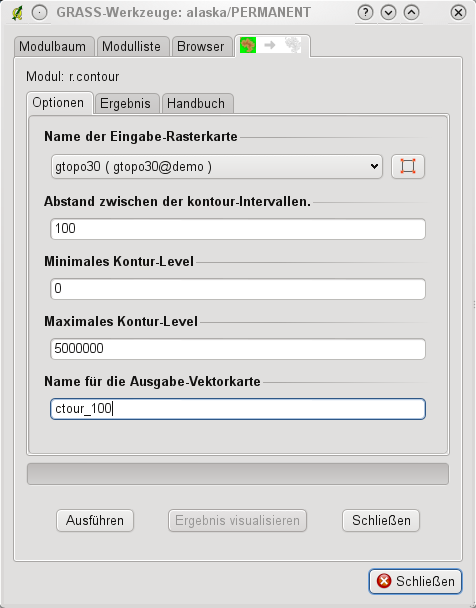
\includegraphics[clip=true, width=0.4\textwidth]{grass_toolbox_rcontour}}
    \hspace{0.5cm}
   \subfloat[r.contour Output] {\label{subfig:grass_toolbox_rcontour2}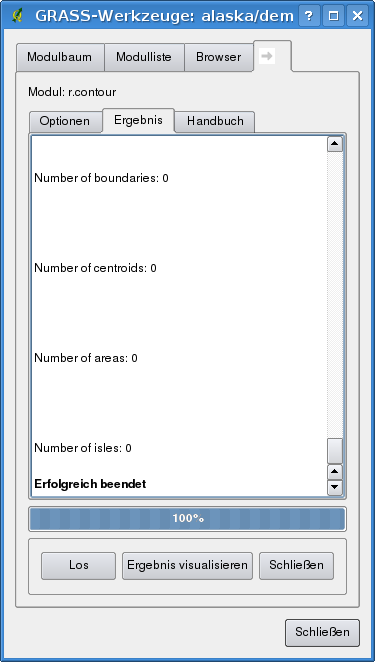
\includegraphics[clip=true, width=0.4\textwidth]{grass_toolbox_rcontour2}}
   \caption{\grass Toolbox r.contour module \nixcaption}\label{fig:grass_toolbox_rcontour}
\end{figure}

% Since this is a large region, it will take a while to display. After it
% finishes rendering, you can open the layer properties window to change the
% line color so that the contours appear clearly over the elevation raster, as
% in \ref{sec:vectorprops}.
Comme il s'agit d'une grande région, cela prendra un certain temps à s'afficher. 
Une fois l'affichage terminé, voujspouvez ouvrir la fenêtre propriétés de la couche pour changer la couleur des cpourbes de niveai afin qu'elles apparaissent clairement au dessus de la couche raster comme au \ref{sec:vectorprops}.

% Next zoom in to a small mountainous area in the center of Alaska.
% Zooming in close you will notice that the contours have sharp corners. \grass
% offers the \classname{v.generalize} tool to slightly alter vector maps while
% keeping their overall shape. The tool uses several different algorithms with
% different purposes. Some of the algorithms (i.e. Douglas Peuker and Vertex
% reduction) simplify the line by removing some of the vertices. The resulting
% vector will load faster. This process will be used when you have a highly
% detailed vector, but you are creating a very small scale map, so the detail
% is unnecessary. 

Zoomez sur une petite région montagneuse du centre de l'Alaska. Avec un fort zoom, vous constaterez que les courbes de niveau sont constitués de lignes brisées avec des angles vifs. \grass offre le possibilité de généraliser les cartes vecteurs à l'aide de l'outil \classname{v.generalize}, tout en conservant leur forme générale. L'outil utilise différents algorithmes ayant différents objectifs. Certains de ces algorithmes (par exemple : Douglas Peuker et réduction de vertex) simplifient les lignes en supprimant des vertex. La couche simplifiée se chargera plus rapidement. cette commande peut être utilisée lorsque vous avez une couche vecteur très détaillée et que vous créez une carte à petite échelle. les détails ne sont donc pas nécessaires.

%\begin{Tip}\caption{\textsc{The simplify tool}}\index{\grass!display results}
\begin{Tip}\caption{\textsc{l'outil de simplification}}\index{\grass!afficher les résultats}
% \qgistip{Note that the \qg fTools plugin has a \dropmenuopt{Simplify geometries} tool that works just like the \grass \classname{v.generalize}
% Douglas-Peuker algorithm. 
Vous remarquerez que fTools dispose aussi d'un outil de simplification \dropmenuopt{Simplifier la géometrie} qui fonctionne comme l'algorithme Douglas-Peuker de \grass \classname{v.generalize}.
\end{Tip}

% However, the purpose of this example is different. The contour lines created
% by r.contour have sharp angles that should be smoothed. Among the
% \classname{v.generalize} algorithms there is Chaikens which does just that
% (also Hermite splines). Be aware that these algorithms can \textbf{add}
% additional vertices to the vector, causing it to load even more slowly.
Cependant, le but de cet exemple est différent. Les courbes de niveau créées avec r.contour ont des angles vifs qui devront être lissés. Parmi les algorithmes de \classname{v.generalize}, il y a l'algorithme de Chaikens qui fait justement ça (comme Hermite splines) . Gardez à l'esprit que ces algorithmes peuvent \textbf{ajouter} des sommets supplémentaires au vecteur, l'amenant à se charger encore plus lentement.

\begin{itemize}[label=--]
% \item Open the \grass toolbox and double click the categories Vector -> Develop map -> Generalization, then click on the \classname{v.generalize} module to open its options window. 
\item Ouvrez la boite à outils \grass et double cliquez sur Vecteur -> Développer la carte -> Généralisation. Cliquez alors sur le module \classname{v.generalize} pour ouvrir sa fenêtre d'options
%\item Check that the \usertext{ctour\_100} vector appears as the \inputtext{Name of input vector}{ctour\_100}.
\item Vérifier que la couche vecteur \usertext{ctour\_100} apparait dans le champs\\ \inputtext{Nom de la couche vectorielle en entrée}{ctour\_100}
%\item From the list of algorithms choose Chaiken's. Leave all other options at their default, and scroll down to the last row to enter the \inputtext{Name for output vector map}{ctour\_100\_smooth}, and click \button{Run}.
\item Dans la liste des algorithmes choisissez Chaiken. Laisser les autres options par défault et descendez à la dernière ligne pour donner le nom de la couche d'information à créer  \inputtext{Nom de la couche vectorielle en sortie}{ctour\_100\_smooth}, et cliquer sur \button{Lancer}
% \item The process takes several moments. Once \usertext{Successfully finished} appears in the output windows, click \button{Vue} and then
% \button{close}.
\item Cela peut prendre plusieurs minutes. Lorsque le texte \usertext{Terminé avec succès} apparait, cliquez sur le bouton \button{Vue} et ensuite sur \button{Fermer}
%\item You may change the color of the vector to display it clearly on the raster background and to contrast with the original contour lines. You will notice that the new contour lines have smoother corners than the original while staying faithful to the original overall shape.
\item Vous pouvez changer la couleur de cette couche vecteur pour qu'elle apparaisse clairement sur le raster et qu'elle contraste aussi avec la couche de départ.Vous remarquerez que les nouvelles courbes de niveau ont des angles plus arrondis que l'original tout en restant fidèle à la forme globale d'origine
\end{itemize}

\begin{figure}[ht]
 \begin{center}
 %%\caption{\grass module v.generalize to smooth a vector map \nixcaption}\label{fig:grass_toolbox_vgeneralize}
 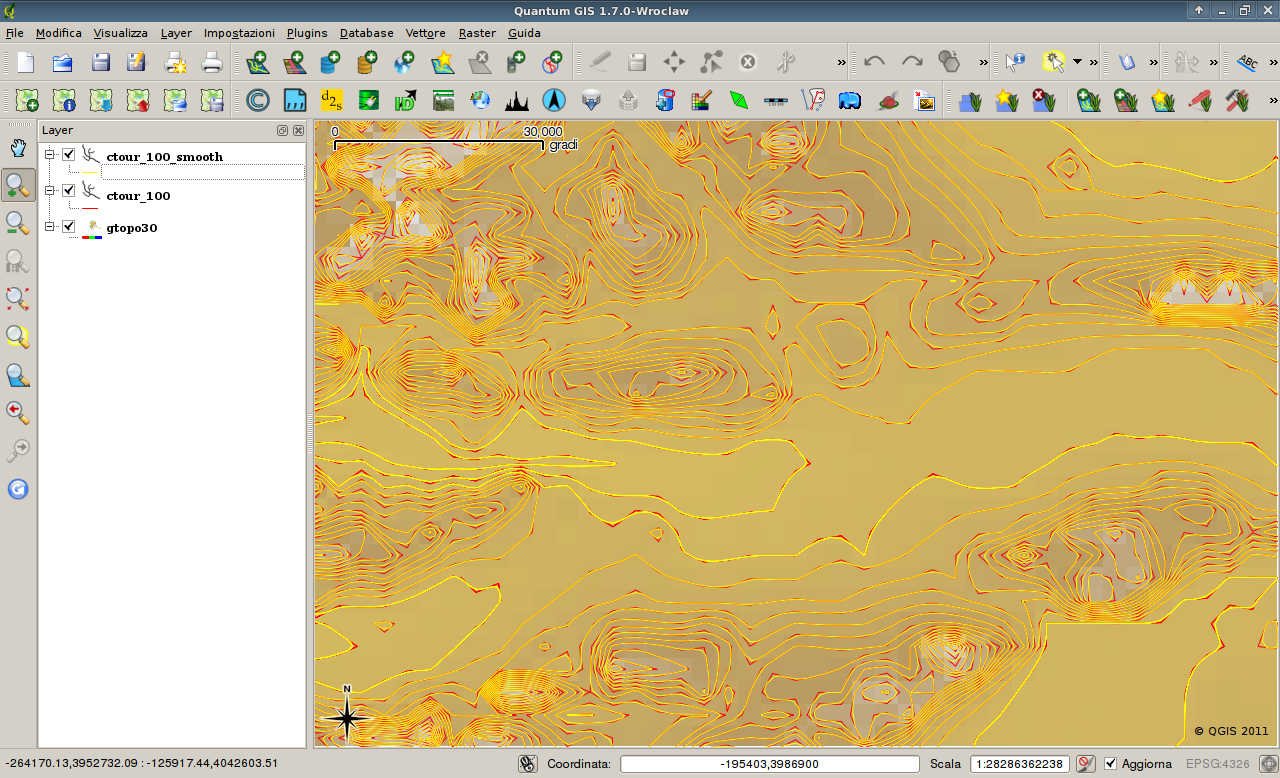
\includegraphics[clip=true, width=12cm]{grass_toolbox_vgeneralize}
 \caption{Module \grass v.generalize pour généraliser les couches vecteurs \nixcaption}\label{fig:grass_toolbox_vgeneralize}
 \end{center}
\end{figure}

%\begin{Tip}\caption{\textsc{Other uses for r.contour}}\index{\grass!toolbox}
\begin{Tip}\caption{\textsc{Autres utilisations de r.contour}}\index{\grass!boîte à outils}
% \qgistip{The procedure described above can be used in other equivalent
% situations. If you have a raster map of precipitation data, for example, then
% the same method will be used to create a vector map of isohyetal (constant
% rainfall) lines
La procédure décrite ci-dessus peut être utilisée dans d'autres cas. Si vous disposez d'une couche d'informations raster representant des précipitations, par exemple, vous pouvez utiliser la même méthode pour créer des isohyètes (lignes reliant des points d'égales quantités de précipitations).
\end{Tip}  

%\minisec{Creating a Hillshade 3D effect}
\minisec{Créer un ombrage avec effet 3D}

% Several methods are used to display elevation layers and give a 3D effect to
% maps. The use of contour lines as shown above is one popular method often
% chosen to produce topographic maps. Another way to display a 3D effect is by
% hillshading. The hillshade effect is created from a DEM (elevation) raster by
% first calculating the slope and aspect of each cell, then simulating the
% sun's position in the sky and giving a reflectance value to each cell. Thus
% you get sun facing slopes lighted and the slopes facing away from the sun (in
% shadow) are darkened.

Différentes méthode sont utilisées pour afficher les modèles numérique de terrain et donner un effet 3D au carte.
L'utilisation de courbe de niveau comme décrit ci-dessus est un des moyens de souvent utilisés pour produire des cartes topographiques.
Un autre moyen de rendre cet effet 3D est d'utiliser l'ombrage. L'ombrage est créé à partir du modèle numérique de terrain (MNT) en calculant d'abord les pentes et les expositions et ensuite en simulant la position du soleil dans le ciel ce qui donne à chaque cellule une valeur de réflectance. Les pentes éclairées par le soleil sont plus claires et les pentes à l'abri du soleil sont plus sombres.

\begin{itemize}[label=--]
% \item Begin this example by loading the \usertext{gtopo30} elevation raster.
% Start the \grass toolbox and under the Raster category double click to open Spatial
% analysis -> Terrain analysis.
\item Commencez par ouvrir la couche raster \usertext{gtopo30}. Ouvrez la boite à outils \grass et dans la catégorie Raster double cliquez sur Spatial
analysis -> Terrain analysis.
%\item Then click \classname{r.shaded.relief} to open the module. 
\item Cliquez ensuite sur \classname{r.shaded.relief} pour lancer le module.
% \item Change the \inputtext{azimuth angle}{270} to 315. Enter \usertext{gtopo30\_shade} for the new hillshade raster, and click 
\button{run}. 
\item Changer \inputtext{azimuth angle}{270} par 315. Saisissez \usertext{gtopo30\_shade} comme nom pour la nouvelle couche d'ombrage et cliquez sur le bouton \button{Lancer}.

%\item When the process completes, add the hillshade raster to the map. You should see it displayed in grayscale.
\item Quand le calcul est terminé, ajoutez le raster ombrage à la fenêtre carte. Normalement, il devrait s'afficher en niveau de gris.
% \item To view both the hill shading and the colors of the \usertext{gtopo30} together shift the hillshade map below the \usertext{gtopo30} map in the table of contents, then open the \dropmenuopt{Properties} window of \usertext{gtopo30}, switch to the \tab{transparency} tab and set its transparency level to about 25\%.
\item Pour voir les 2 couches d'informations ombrage et \usertext{gtopo30} en même temps, placez la couche ombrage sous la couche \usertext{gtopo30} dans le gestionnaire de couches et ouvrez la fenêtre propriétés de la couche \usertext{gtopo30}, allez sur l'onglet "Transparence" et fixé la transparence à environ 25\%
\end{itemize}

% You should now have the \usertext{gtopo30} elevation with its colormap and transparency setting displayed \textbf{above} the grayscale hillshade map. In
% order to see the visual effects of the hillshading, turn off the \usertext{gtopo30\_shade} map, then turn it back on.
Vous devriez maintenant avoir la couche \usertext{gtopo30} en couleur et en transparence, affiché au dessus \textbf{above}, la couche ombrage en niveau de gris.

%\minisec{Using the \grass shell}
\minisec{Utiliser la console \grass}
\begin{figure}[ht]
 \begin{center}
% \caption{The \grass shell, r.shaded.relief module \nixcaption}\label{fig:grass_toolbox_shell}

 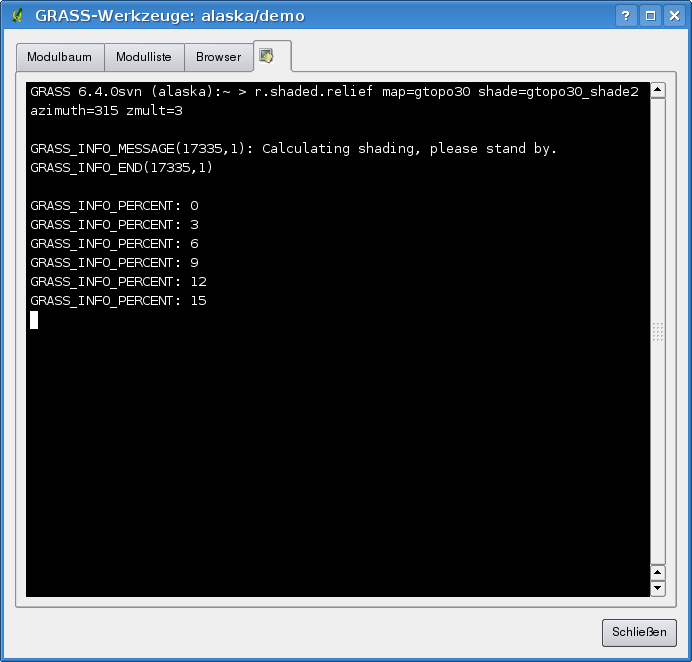
\includegraphics[clip=true, width=10cm]{grass_toolbox_shell}
 \caption{La console \grass,module r.shaded.relief \nixcaption}\label{fig:grass_toolbox_shell}
 \end{center}
\end{figure}
% The \grass plugin in \qg is designed for users who are new to \grass, and not familiar with all the modules and options. As such, some modules in the
% toolbox do not show all the options available, and some modules do not appear at all. The \grass shell (or console) gives the user access to those
% additional \grass modules that do not appear in the toolbox tree, and also to some additional options to the modules that are in the toolbox with the
% simplest default parameters. This example demonstrates the use of an additional option in the \classname{r.shaded.relief} module that was shown above.
L'extension Grass dans \qg est faite pour les utilisateurs ne connaissant pas \grass et qui ne sont pas familiers avec les modules et les options.
Certains modules dans la boite à outils n'apparaissent pas avec toutes les options possibles et certains n'apparaissent pas du tout. La console \grass donne accès à ces modules additionnels qui n'apparaissent pas dans la boite à outils et aussi aux options des modules qui n'apparaissent que de façon simplifiés dans la boite à outils. Cet exemple montre l'utilisation des options supplémentaires du module \classname{r.shaded.relief} utilisé ci-dessus.



% The module \classname{r.shaded.relief} can take a parameter \usertext{zmult} which multiplies the elevation values relative to the X-Y coordinate units so
% that the hillshade effect is even more pronounced. 
Le module \classname{r.shaded.relief} possède un paramètre \usertext{zmult} qui multiplie la valeur de l'altitude (exprimé dans la même unité que les coordonnées X - Y) ce qui a pour effet d'accentuer/exagérer le relief.

\begin{itemize}[label=--]
% \item Load the \usertext{gtopo30} elevation raster as above, then start the \grass toolbox and click on the \grass shell. In the shell window type the
% command:\linebreak \usertext{r.shaded.relief map=gtopo30 shade=gtopo30\_shade2 azimuth=315 zmult=3} \linebreak and press \keystroke{Enter}.
\item Ouvrez le raster \usertext{gtopo30} comme ci-dessus, et lancez la boite à outils \grass et ouvrez la console \grass. Dans la console, entrez la ligne suivante:\linebreak \usertext{r.shaded.relief map=gtopo30 shade=gtopo30\_shade2 azimuth=315 zmult=3} \linebreak et pressez \keystroke{Enter}.

% \item After the process finishes shift to the \tab{Browse} tab and double click on the new \usertext{gtopo30\_shade2} raster to display in \qg. 
% \item As explained above, shift the shaded relief raster below the gtopo30 raster in the Table of Contents, then check transparency of the colored
%gtopo30 layer. You should see that the 3D effect stands out more strongly compared to the first shaded relief map.
\item Une fois le calcul terminé, allez sur l'onglet \tab{Browse} et doubel-cliquez sur le nouveau raster \usertext{gtopo30\_shade2} pour l'afficher dans \qg.
\end{itemize}

\begin{figure}[p]
 \begin{center}
 %\caption{Displaying shaded relief created with the \grass module r.shaded.relief \nixcaption}\label{fig:grass_toolbox_shadedrelief}

 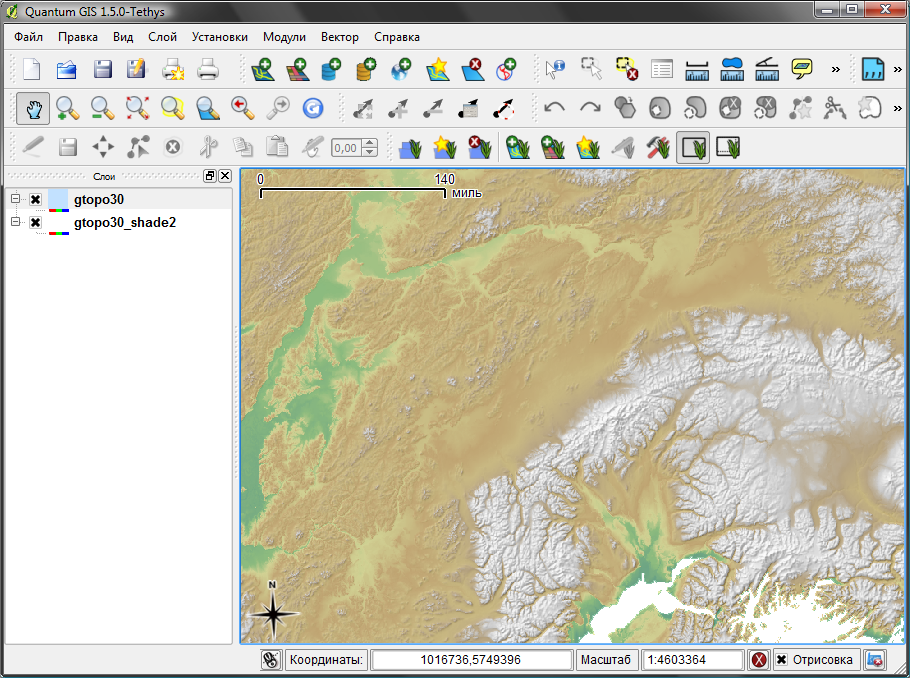
\includegraphics[clip=true, width=12cm]{grass_toolbox_shadedrelief}
  \caption{Afficher une couche d'ombrage créée avec le module \grass r.shaded.relief \nixcaption}\label{fig:grass_toolbox_shadedrelief}
 \end{center}
\end{figure}

%\minisec{Raster statistics in a vector map}
\minisec{Statistiques raster avec des couches vectorielles}

%The next example shows how a \grass module can aggregate raster data and add columns of statistics for each polygon in a vector map. 
L'exemple suivant comment un module \grass peut aggréger des données et ajouter des colonnes de statistiques pour des polygones d'un couche vecteur.

\begin{itemize}[label=--]
%\item Again using the Alaska data, refer to \ref{sec:import_loc_data} to import the trees shapefile from the \usertext{vmap0\_shapefiles} directory
%into \grass.
\item Encore une fois, nous allons utiliser le jeu de  données Alaska. Référez vous à \ref{sec:import_loc_data} pour importer les shapefiles contenus dans le répetoire \usertext{vmap0\_shapefiles} dans \grass.
% \item Now an intermediary step is required: centroids must be added to the imported trees map to make it a complete \grass area vector (including both
% boundaries and centroids). 
\item Un étape intermédiaire est nécessaire: des centroïdes doivent importés afin d'avoir une couche \grass vecteur complète (incluant les contours et les centroïdes)
%\item From the toolbox choose Vector -> Manage features, and open the module \classname{v.centroids}.
\item Dans la boite à outils choisissez Vector -> Manage features,et ouvrez le module \classname{v.centroids}.
%\item Enter as the \inputtext{output vector map}{\usertext{forest\_areas}} and run the module. 
\item Entrez comme nom de couche en sortie \inputtext{output vector map}{\usertext{forest\_areas}} et lancez le module.
% \item Now load the \usertext{forest\_areas} vector and display the types of forests - deciduous, evergreen, mixed - in different colors: In the layer
% \dropmenuopt{Properties} window, \tab{symbology} tab, choose \selectstring{Legend type}{Unique value} and set the \inputtext{Classification field}{VEGDESC} to VEGDESC. (Refer to the explanation of the symbology tab \ref{sec:symbology} in the vector section).
\item Maintenant ouvrez la couche vecteur \usertext{forest\_areas} et affichez les types de forêts avec différentes couleurs : caduques, sempervirens, mélangés. Dans la fenêtre\\ \dropmenuopt{Propriétés}, onglet \tab{symbologie} , choisissez \selectstring{Type de légende}{Valeur unique} comme type de thématisation et le champ de \inputtext{Classification field}{VEGDESC} au champ VEGDESC. (Reportez vous aux explications de l'onglet Symbologie \ref{sec:symbology} dans la partie vecteur).

%\item Next reopen the \grass toolbox and open Vector -> Vector update by other maps.
\item Réouvrez la boite à outils \grass et ouvrez Vector -> Vector update par d'autres couches
% \item Click on the \classname{v.rast.stats} module. Enter \usertext{gtopo30}, and \usertext{forest\_areas}. 
\item Cliquez sur le module \classname{v.rast.stats}. Saisissez \usertext{gtopo30}, et \usertext{forest\_areas}.
% \item Only one additional parameter is needed: Enter \inputtext{column prefix}{\usertext{elev}}, and click \button{Lancer}. This is a computationally
% heavy operation which will run for a long time (probably up to two hours).
\item Seulement un paramètre additionnel est requis : Entrez  \inputtext{column prefix}{\usertext{elev}}, et cliquez sur le bouton \button{Lancer}. C'est un opération lourde qui peut durer longtemps.
% \item Finally open the \usertext{forest\_areas} attribute table, and verify that several new columns have been added including \usertext{elev\_min},
% \usertext{elev\_max}, \usertext{elev\_mean} etc. for each forest polygon.
\item Finallement, ouvrez la table attributaire de \usertext{forest\_areas}, et vérifiez que plusieurs nouvelles colonnes ont étés ajoutées dont \usertext{elev\_min},\usertext{elev\_max}, \usertext{elev\_mean}, etc., pour chaque polygones de forêt.
\end{itemize}

%\subsection{Working with the \grass LOCATION browser} \index{\grass!toolbox!Browser}
\subsection{Travailler avec le navigateur \grass} \index{\grass!boîte à outils!navigateur}

% Another useful feature inside the \grass Toolbox is the \grass \filename{LOCATION} browser. In Figure~\ref{fig:grass_mapset_browser} you 
% can see the current working \filename{LOCATION} with its \filename{MAPSETs}.
Une autre fonctionnalité utile dans la boîte à outils \grass est le navigateur de \filename{SECTEUR} \grass. Sur la figure~\ref{fig:grass_mapset_browser}
vous pouvez voir le \filename{SECTEUR} en cours  avec ses \filename{Jeux de Données}.

% In the left browser windows you can browse through all \filename{MAPSETs} 
% inside the current \filename{LOCATION}. The right browser window shows some 
% meta information for selected raster or vector layers, e.g. resolution, 
% bounding box, data source, connected attribute table for vector data and a 
% command history.
Dans la partie gauche de la fenêtre vous pouvez naviguer dans tous les \filename{Jeux de Données} du \filename{SECTEUR} courant. La partie droite de la fenêtre affiche des informations sur le raster ou le vecteur sélectionné, tel que la résolution, l'emprise, la source des données, les tables attributaires pour les vecteurs et un historique des commandes.

\begin{figure}[ht]
 \begin{center}
 %\caption{\grass LOCATION browser \nixcaption}\label{fig:grass_mapset_browser}
 
 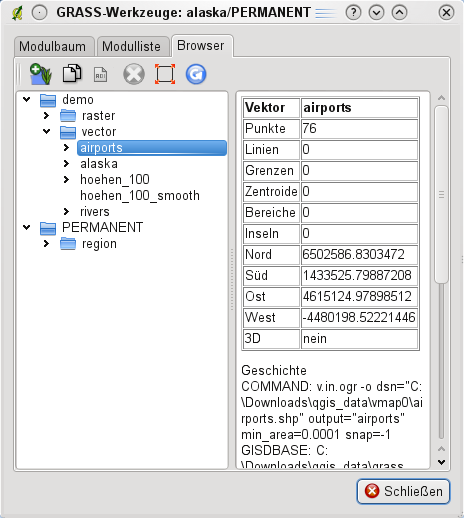
\includegraphics[clip=true,width=10cm]{grass_mapset_browser}
 \caption{Navigateur de SECTEUR \grass \nixcaption}\label{fig:grass_mapset_browser}
 \end{center}
\end{figure}

%The toolbar inside the \tab{Browser} tab offers following tools to manage 
%the selected \filename{LOCATION}:
La barre d'outils de l'onglet \tab{Parcourir} donne accès à des outils de gestion du \filename{SECTEUR} sélectionné :

\begin{itemize}[label=--]
% \item \toolboxtwo{grass_add_map}{Add selected map to canvas}
% \item \toolboxtwo{grass_copy_map}{Copy selected map}
% \item \toolboxtwo{grass_rename_map}{Rename selected map}
% \item \toolboxtwo{grass_delete_map}{Delete selected map}
% \item \toolboxtwo{grass_set_region}{Set current region to selected map}
% \item \toolboxtwo{grass_refresh}{Refresh browser window}
\item \toolboxtwo{grass_add_map}{ Ajoute la carte sélectionnée à la carte \qg}
\item \toolboxtwo{grass_copy_map}{Copie la carte sélectionnée}
\item \toolboxtwo{grass_rename_map}{Renomme la carte sélectionnée}
\item \toolboxtwo{grass_delete_map}{Efface la carte sélectionnée}
\item \toolboxtwo{grass_set_region}{Région courante réglée sur la carte choisie}
\item \toolboxtwo{grass_refresh}{Rafraîchir}
\end{itemize}

% The \toolboxtwo{grass_rename_map}{Rename selected map} and \toolboxtwo{grass_delete_map}{Delete selected map} only work with maps inside 
% your currently selected \filename{MAPSET}. All other tools also work with raster and vector layers in another \filename{MAPSET}.
Les commandes \toolboxtwo{grass_rename_map}{Renommer la carte sélectionnée} et \toolboxtwo{grass_delete_map}{Effacer la carte sélectionnée} ne fonctionnent qu'avec les cartes présente dans votre \filename{Jeu de Données} sélectionné. Tous les autres outils fonctionnent aussi avec les autres \filename{Jeux de Données}.

\subsection{Paramètrer la boite à outils \grass} \index{\grass!toolbox!customize}
\label{sec:toolbox-customizing}

% Nearly all \grass modules can be added to the \grass toolbox. A XML 
% interface is provided to parse the pretty simple XML files which configures 
% the modules appearance and parameters inside the toolbox.
Pratiquement tous les modules \grass peuvent être ajoutés à la boîte à outils. Une interface XML est fournie pour analyser les fichiers XML 
très simple qui configurent l'apparence et les paramètres des modules dans la boîte à outils.

%A sample XML file for generating the module \usertext{v.buffer} (v.buffer.qgm) looks like this:
Un exemple de fichier XML pour le module \usertext{v.buffer} (v.buffer.qgm) est donné ci-dessous :
\begin{verbatim}
<?xml version="1.0" encoding="UTF-8"?>
<!DOCTYPE qgisgrassmodule SYSTEM "http://mrcc.com/qgisgrassmodule.dtd">

<qgisgrassmodule label="Vector buffer" module="v.buffer">
        <option key="input" typeoption="type" layeroption="layer" />
        <option key="buffer"/>
        <option key="output" />
</qgisgrassmodule>
\end{verbatim}
%
%The parser reads this definition and creates a new tab inside the toolbox when you select the module. A more detailed description for adding new  modules, changing the modules group, etc. can be found on the \qg wiki at \\\url{http://wiki.qgis.org/qgiswiki/Adding\_New\_Tools\_to\_the\_\grass\_Toolbox}.
L'analyseur lit cette définition et crée un nouvel onglet à l'intérieur de la boîte à outils lorsque vous sélectionnez le module. Une description plus détaillée pour ajouter des modules, changer le groupe des modules, etc. est disponible sur le wiki \qg à l'adresse \url{http://wiki.qgis.org/qgiswiki/Adding_New_Tools_to_the_GRASS_Toolbox}.
